\documentclass[A4paper,man,floatsintext]{apa6}
\usepackage{lmodern}
\usepackage{amssymb,amsmath}
\usepackage{ifxetex,ifluatex}
\usepackage{fixltx2e} % provides \textsubscript
\ifnum 0\ifxetex 1\fi\ifluatex 1\fi=0 % if pdftex
  \usepackage[T1]{fontenc}
  \usepackage[utf8]{inputenc}
\else % if luatex or xelatex
  \ifxetex
    \usepackage{mathspec}
  \else
    \usepackage{fontspec}
  \fi
  \defaultfontfeatures{Ligatures=TeX,Scale=MatchLowercase}
\fi
% use upquote if available, for straight quotes in verbatim environments
\IfFileExists{upquote.sty}{\usepackage{upquote}}{}
% use microtype if available
\IfFileExists{microtype.sty}{%
\usepackage{microtype}
\UseMicrotypeSet[protrusion]{basicmath} % disable protrusion for tt fonts
}{}
\usepackage{hyperref}
\hypersetup{unicode=true,
            pdftitle={A multilab registered replication of the attentional SNARC effect},
            pdfauthor={Lincoln J Colling, Dénes Szűcs, Damiano De Marco, Krzysztof Cipora, Rolf Ulrich, Hans-Christoph Nuerk, Mojtaba Soltanlou, Donna Bryce, Sau-Chin Chen, Philipp Alexander Schroeder, Dion T Henare, Christine K Chrystall, Paul M Corballis, Daniel Ansari, Celia Goffin, H Moriah Sokolowski, Peter JB Hancock, Ailsa E Millen, Stephen RH Langton, Kevin J Holmes, Mark S Saviano, Tia A Tummino, Oliver Lindemann, Rolf A Zwaan, Jiří Lukavský, Adéla Becková, Marek A Vranka, Simone Cutini, Irene Cristina Mammarella, Claudio Mulatti, Raoul Bell, Axel Buchner, Laura Mieth, Jan Philipp Röer, Elise Klein, Stefan Huber, Korbinian Moeller, Brenda Ocampo, Juan Lupiáñez, Javier Ortiz-Tudela, Juanma De la fuente, Julio Santiago, Marc Ouellet, Edward M Hubbard, Elizabeth Y Toomarian, Remo Job, Barbara Treccani, \& Blakeley B McShane},
            pdfborder={0 0 0},
            breaklinks=true}
\urlstyle{same}  % don't use monospace font for urls
\usepackage[style=apa]{biblatex}

\addbibresource{cited.bib}
\usepackage{graphicx,grffile}
\makeatletter
\def\maxwidth{\ifdim\Gin@nat@width>\linewidth\linewidth\else\Gin@nat@width\fi}
\def\maxheight{\ifdim\Gin@nat@height>\textheight\textheight\else\Gin@nat@height\fi}
\makeatother
% Scale images if necessary, so that they will not overflow the page
% margins by default, and it is still possible to overwrite the defaults
% using explicit options in \includegraphics[width, height, ...]{}
\setkeys{Gin}{width=\maxwidth,height=\maxheight,keepaspectratio}
\IfFileExists{parskip.sty}{%
\usepackage{parskip}
}{% else
\setlength{\parindent}{0pt}
\setlength{\parskip}{6pt plus 2pt minus 1pt}
}
\setlength{\emergencystretch}{3em}  % prevent overfull lines
\providecommand{\tightlist}{%
  \setlength{\itemsep}{0pt}\setlength{\parskip}{0pt}}
\setcounter{secnumdepth}{0}
% Redefines (sub)paragraphs to behave more like sections
\ifx\paragraph\undefined\else
\let\oldparagraph\paragraph
\renewcommand{\paragraph}[1]{\oldparagraph{#1}\mbox{}}
\fi
\ifx\subparagraph\undefined\else
\let\oldsubparagraph\subparagraph
\renewcommand{\subparagraph}[1]{\oldsubparagraph{#1}\mbox{}}
\fi

%%% Use protect on footnotes to avoid problems with footnotes in titles
\let\rmarkdownfootnote\footnote%
\def\footnote{\protect\rmarkdownfootnote}


  \title{A multilab registered replication of the attentional SNARC effect}
    \author{\textbf{Lincoln J Colling}\textsuperscript{1}, \textbf{Dénes
Szűcs}\textsuperscript{1}, Damiano De Marco\textsuperscript{1, 12},
Krzysztof Cipora\textsuperscript{2}, Rolf Ulrich\textsuperscript{2},
Hans-Christoph Nuerk\textsuperscript{2}, Mojtaba
Soltanlou\textsuperscript{2}, Donna Bryce\textsuperscript{2}, Sau-Chin
Chen\textsuperscript{3}, Philipp Alexander Schroeder\textsuperscript{4},
Dion T Henare\textsuperscript{5}, Christine K
Chrystall\textsuperscript{5}, Paul M Corballis\textsuperscript{5},
Daniel Ansari\textsuperscript{6}, Celia Goffin\textsuperscript{6}, H
Moriah Sokolowski\textsuperscript{6}, Peter JB
Hancock\textsuperscript{7}, Ailsa E Millen\textsuperscript{7}, Stephen
RH Langton\textsuperscript{7}, Kevin J Holmes\textsuperscript{8}, Mark S
Saviano\textsuperscript{8}, Tia A Tummino\textsuperscript{8}, Oliver
Lindemann\textsuperscript{9}, Rolf A Zwaan\textsuperscript{9}, Jiří
Lukavský\textsuperscript{10}, Adéla Becková\textsuperscript{11}, Marek A
Vranka\textsuperscript{11}, Simone Cutini\textsuperscript{12}, Irene
Cristina Mammarella\textsuperscript{12}, Claudio
Mulatti\textsuperscript{12}, Raoul Bell\textsuperscript{13}, Axel
Buchner\textsuperscript{13}, Laura Mieth\textsuperscript{13}, Jan
Philipp Röer\textsuperscript{14, 2}, Elise Klein\textsuperscript{15},
Stefan Huber\textsuperscript{15}, Korbinian
Moeller\textsuperscript{15,2}, Brenda Ocampo\textsuperscript{16}, Juan
Lupiáñez\textsuperscript{17}, Javier Ortiz-Tudela\textsuperscript{17},
Juanma De la fuente\textsuperscript{17}, Julio
Santiago\textsuperscript{17}, Marc Ouellet\textsuperscript{17}, Edward M
Hubbard\textsuperscript{18}, Elizabeth Y Toomarian\textsuperscript{18},
Remo Job\textsuperscript{19}, Barbara Treccani\textsuperscript{19}, \&
Blakeley B McShane\textsuperscript{20}}
    \date{}
  
\shorttitle{Replication of the attentional SNARC effect}
\affiliation{
\vspace{0.5cm}
\textsuperscript{1} Department of Psychology, University of Cambridge\\\textsuperscript{2} Department of Psychology, University of Tübingen\\\textsuperscript{3} Department of Human Development and Psychology, Tzu-Chi University\\\textsuperscript{4} Department of Psychiatry and Psychotherapy, University of Tübingen\\\textsuperscript{5} School of Psychology, University of Auckland\\\textsuperscript{6} Department of Psychology \& Brain and Mind Institute, The University of Western Ontario\\\textsuperscript{7} Psychology, Faculty of Natural Sciences, University of Stirling, Stirling, UK\\\textsuperscript{8} Department of Psychology, Colorado College\\\textsuperscript{9} Department of Psychology, Education \& Child Studies, Erasmus University Rotterdam, Netherlands\\\textsuperscript{10} Institute of Psychology of the Czech Academy of Sciences\\\textsuperscript{11} Department of Psychology, Faculty of Arts, Charles University\\\textsuperscript{12} Department of Developmental Psychology, University of Padova\\\textsuperscript{13} Department of Experimental Psychology, Heinrich Heine University Düsseldorf\\\textsuperscript{14} Department of Psychology and Psychotherapy, Witten/Herdecke University\\\textsuperscript{15} Leibniz-Institut für Wissensmedien, Tübingen\\\textsuperscript{16} School of Psychology, The University of Queensland\\\textsuperscript{17} Research Center for Mind, Brain, and Behavior, University of Granada\\\textsuperscript{18} Department of Educational Psychology, University of Wisconsin-Madison\\\textsuperscript{19} Department of Psychology and Cognitive Science, University of Trento\\\textsuperscript{20} Kellogg School of Management, Northwestern University}
\usepackage{csquotes}
\usepackage{upgreek}
\captionsetup{font=singlespacing,justification=justified}

\usepackage{longtable}
\usepackage{lscape}
\usepackage{multirow}
\usepackage{tabularx}
\usepackage[flushleft]{threeparttable}
\usepackage{threeparttablex}

\newenvironment{lltable}{\begin{landscape}\begin{center}\begin{ThreePartTable}}{\end{ThreePartTable}\end{center}\end{landscape}}

\makeatletter
\newcommand\LastLTentrywidth{1em}
\newlength\longtablewidth
\setlength{\longtablewidth}{1in}
\newcommand{\getlongtablewidth}{\begingroup \ifcsname LT@\roman{LT@tables}\endcsname \global\longtablewidth=0pt \renewcommand{\LT@entry}[2]{\global\advance\longtablewidth by ##2\relax\gdef\LastLTentrywidth{##2}}\@nameuse{LT@\roman{LT@tables}} \fi \endgroup}


\usepackage{lineno}

\linenumbers
\renewcommand\appendixname{Supplementary Results}
\usepackage{subcaption}
\usepackage{caption}
\usepackage{makecell}
\DeclareLanguageMapping{english}{english-apa}
\DeclareBibliographyCategory{asterisk}
\renewbibmacro*{begentry}{\ifcategory{asterisk}{\ensuremath{\ast}}{}}
\newcommand*{\nocitemeta}[1]{\nocite{#1}\addtocategory{asterisk}{#1}}
\usepackage{fontspec}
\setmainfont{Tinos}
\usepackage{float}
\floatplacement{figure}{htp}

\authornote{

Correspondence concerning this article should be addressed to
\textbf{Dénes Szűcs}, Downing Street, CB2 3EB, Cambridge, UK. E-mail:
\href{mailto:ds377@cam.ac.uk}{\nolinkurl{ds377@cam.ac.uk}}}

\abstract{
The attentional Spatial-Numerical Association of Response Codes
(att-SNARC) effect (Fischer et al., 2003; Nature Neuroscience)---the
finding that participants are quicker to detect left-side targets when
the targets are preceded by small numbers and quicker to detect
right-side targets when they are preceded by large numbers---has been
used as evidence for \emph{embodied} number representations and to allow
for strong claims about the link between number and space (e.g., a
mental number line). We attempted to replicate Study 2 of Fischer et al.
(2003) by collecting data from 1105 participants across seventeen labs.
Across all 1105 participants and four ISI conditions, the proportion of
times the direction of the observed effect was consistent with the
original effect was 0.50. Further, the effects we observed both within
and across labs were minuscule and incompatible with those observed in
Fischer et al. (2003). Given this, we conclude that we have
\emph{failed} to replicate the effect reported by Fischer et al. (2003).
In addition, our analysis of several participant-level moderators
(finger counting preferences, reading/writing direction experience,
handedness, and mathematics fluency and mathematics anxiety) revealed no
substantial moderating effects. Our results demonstrate that the
att-SNARC effect cannot be used as evidence to support the strong claims
about the link between number and space discussed above


}

\usepackage{amsthm}
\newtheorem{theorem}{Theorem}[section]
\newtheorem{lemma}{Lemma}[section]
\theoremstyle{definition}
\newtheorem{definition}{Definition}[section]
\newtheorem{corollary}{Corollary}[section]
\newtheorem{proposition}{Proposition}[section]
\theoremstyle{definition}
\newtheorem{example}{Example}[section]
\theoremstyle{definition}
\newtheorem{exercise}{Exercise}[section]
\theoremstyle{remark}
\newtheorem*{remark}{Remark}
\newtheorem*{solution}{Solution}
\begin{document}
\maketitle

\section{Introduction}\label{introduction}

A foundational issue in cognitive science is the question of how we
\emph{represent} concepts. Classical approaches to cognitive science,
exemplified by Fodor's \autocite*{Fodor1975} \enquote{language of
thought} and Newell and Simon's \autocite*{Newell1976} \enquote{physical
symbol systems} hypothesis, view representations as abstract or amodal
and as distinct from sensorimotor processing. In contrast to these
traditional views, a range of other views that go under labels such as
\enquote{embodied}, \enquote{situated}, or \enquote{grounded} cognition
argue that representations (i) are intimately linked to sensorimotor
processing \autocite[see, e.g.,][ for an overview]{Wilson2002six}; (ii)
are analogue rather than symbolic; and (iii) represent by in some sense
resembling their targets \autocites[e.g.,
see][]{Gladzijewski2017}{Williams2018}.

One area of research that has provided a wealth of empirical findings
valuable for debates about the nature of concept representation has been
numerical cognition. In fact, \textcite{Fischer2011em} have referred to
numerical cognition as the \enquote{prime example of embodied
cognition}. In particular, \textcite{Fischer2011em} point to tasks
examining spatial-numerical associations to make their case.

Researchers have long reasoned that numbers might be represented in a
spatially organised manner \autocite{Galton:1880na}, for example, as a
\emph{mental number line} \autocite[e.g.,][]{Restle:1970km}. Key support
for this notion comes from a series of nine experiments conducted by
\textcite{Dehaene:1993fc}. In these experiments,
\textcite{Dehaene:1993fc} asked participants to judge whether the parity
of a number was odd or even, finding that responses to large numbers
were faster when pressing a right-hand key relative to a left-hand key
while the opposite was true for small numbers. They labelled this number
magnitude by response side interaction the Spatial-Numerical Association
of Response Codes (SNARC) effect.

In these parity judgement experiments, there was no standard with which
to compare the presented number. Consequently, whether a particular
number was responded to quicker with the left hand or the right hand was
not determined by the absolute magnitude of the number, but by the
relative magnitude of the number within a stimulus set. Thus, the number
five was responded to more quickly with the left hand when appearing in
a set of numbers ranging from four to nine but more quickly with the
right hand when appearing in a set of numbers ranging from zero to five
\autocites[e.g.,][]{Dehaene:1993fc}{Fias:1996ms}.

\textcite{Dehaene:1993fc} reported that the effects were neither
dependent on the handedness of participants nor the hand used to make
the response. Instead, they tracked the side of space of the response,
with responses to small numbers being quicker with the right hand when
the participants' hands were crossed \autocite[see,
however,][]{Woods:2006cp}. Nonetheless, \textcite{Dehaene:1993fc} did
report that the effect was dependent on reading/writing direction.
Specifically, while they initially found the effect in French
participants who had experience reading/writing from left to right, the
did not replicate it in a follow-up experiment with Iranian participants
who had experience reading/writing from right to left (see
\textcite{Shaki:2009ch} and \textcite{Zebine}). Together, the results of
the nine experiments reported in \textcite{Dehaene:1993fc} were taken to
support the idea of a mental number line with numbers of increasing
magnitude associated with the left-to-right axis of external space.

While SNARC effects appear to be robust (see \textcite{Wood:2008rev} and
\textcite{Toomarian:2018rev} for recent reviews), the great range of
findings has resulted in some debate about the underlying mechanism(s)
that produce them. One such debate is concerned with whether the SNARC
effect is produced by early, \emph{response-independent} mechanisms or
whether processes at the stage of \emph{response selection} are
responsible. According to theories that place the origin of the SNARC
effect at an early stage, the mere observation of the number should be
sufficient to activate the spatial code because the spatial code is
intimately connected to the numerical representation. Consequently,
these theories make the strongest claims about the link between number
and space. Theories that place the origin of the SNARC effect at the
response selection stage, however, make weaker claims about the
connection between number and space. As \textcite{PecherBoot:2011} note,
if the response selection stage gives rise to the SNARC effect, then no
underlying spatial-numerical representation need be assumed.

Most recent work has tended to support the notion that the response
selection stage is the locus of the SNARC effect. In particular, Keus
and colleagues have used both behavioural \autocite{Keus:2005ho} and
psychophysiological \autocite{Keus:2005jh} evidence to argue in favour
of a later, response-related origin of the SNARC effect. Further support
comes from a computational model that relies on task-dependent
conceptual coding of the number at a stage distinct from the numerical
representation itself \autocite{Gevers:2006model}.

Additional accounts that break the link between number, space, and the
SNARC effect are so-called response polarity-related accounts.
Specifically, \textcite{Proctor:2006jv} argue that on binary
classification tasks, items in the task set are coded as being positive
or negative in polarity. Response selection can then be facilitated when
there is a structural overlap between the polarity of the item (the
number in the case of the SNARC effect) and the response. As with the
model from \textcite{Gevers:2006model}, the account of
\textcite{Proctor:2006jv} does not require any perceptual or conceptual
overlap between the stimulus and the response dimensions for the SNARC
effect to occur. That is, these accounts do not rely on the notion of a
mental number line or sensorimotor-linked representations. A range of
empirical findings support these types of accounts. For example,
\textcite{Santens:2008} found that SNARC-like effects can be produced
when left-right responses are replaced with unimanual close-far
responses, with small numbers associated with close responses and large
numbers associated with far responses. Further, \textcite{Landy:2008}
found that verbal \enquote{Yes} and \enquote{No} responses on a parity
judgement task were facilitated by large numbers and small numbers
respectively.

Finally, still other researchers have argued in favour of a working
memory account of the SNARC effect. For example, in the task reported by
\textcite{vanDijck:2011kk}, participants performed a fruit/vegetable
classification after having been encouraged to store the stimuli as an
ordered set in working memory. This was done by presenting participants
with a sequence of fruit and vegetable names (displayed in the centre of
the screen) before the classification task and then testing them on the
order of the items. A spatial response-compatibility effect emerged with
participants responding faster to items early in the sequence with their
left hand and items later in the sequence with the right hand.
\textcite{vanDijck:2011kk} argue that this working memory account can
also explain why SNARC-like effect emerge for other kinds of ordinal
sequences such as months of the year \autocite{Gevers:2003je} or days of
the week \autocite{Gevers:2004gj} as well as why spatial-numerical
associations can be moderated by giving participants instructions to
associate numbers with positions on a clock-face (1--5 on the right and
6--10 on the left) rather than on a ruler \autocite[1--5 on the left and
6--10 on the right;][]{Bachtold:1998}

Given that several competing accounts of the SNARC effect exist and that
many of the accounts do not require a mental number line, one may doubt
whether spatial-numerical associations provide evidence for anything
like \enquote{embodied} number representations or number representation
that are intimately linked with space. However, there is evidence that
does support an early, response-independent locus for the SNARC effect
and thus does provide support for the notion of a mental number-line and
spatially-linked number representation---the modified version of the
\textcite{Posner} attentional cueing task developed by
\textcite{Fischer:2003ju}. In this study, participants were asked to
detect the appearance of lateralised targets. The target, a white
circle, was preceded by either a small number (1 or 2) or a large number
(8 or 9). Importantly, the digit did not predict the subsequent location
of the target, that is, it was not task-relevant. Instead, the task was
merely to press a single response button when the target appeared
regardless of whether it appeared on the left or the right. Importantly,
not requiring a spatially lateralised response negates the possibility
of any response-related effects. The finding from this paradigm was
consistent with the SNARC effect, as participants were quicker to detect
left-side targets when the targets were preceded by small numbers and
quicker to detect right-side targets when they were preceded by large
numbers, at least for digits and targets that were separated by an
inter-stimulus interval (ISI) between 250 and 1000 ms. This
finding---named the attentional SNARC (att-SNARC) effect---suggests that
viewing numbers alone was able to cue spatial attention either to the
left or the right depending on the magnitude of the number.

Because the att-SNARC effect argues strongly in favour of an early,
response-independent locus for the cause of the SNARC effect, the
att-SNARC effect plays a crucially important role in adjudicating
debates about the origin of the SNARC effect and the nature of number
representations. As a result, the original finding has been extremely
influential (e.g., cited 704 times according to Google Scholar as of 12
September 2019). However, subsequent attempts to replicate the effect
have produced mixed results.

\textcite{Galfano:2006cu} report a statistically significant effect for
right-side targets when the data was collapsed across two ISI conditions
of 500 and 800 ms using a one-tailed test {[}Estimate = 6.5 ms;
\emph{t}(25) = 1.75; \emph{p} = .046 (reported as \emph{p} = .04){]}.
They also report a statistically significant effect for left-side
targets collapsed across the two ISI conditions, but the claimed
statistical significance reflected a reporting error {[}Estimate = 5.5
ms; \emph{t}(25) = 1.59; \emph{p} = .062 (reported as \emph{p} =
.04){]}. Finally, they report an overall estimate (collapsed across the
left and right target locations) of 8 ms for the 500 ms ISI condition
and 4 ms for the ISI 800 ms condition, but the reporting is such that
the corresponding variances or test statistics for these estimates
cannot be obtained.

In addition, \textcite{Dodd:2008dv} report a statistically significant
effect when the data was collapsed across three ISI conditions between
250 and 750 ms and across both left and right target locations, but
again the claimed statistical significance reflected a reporting error
{[}Estimate = 5.5 ms; \emph{F}(1,29) = 4.05; \emph{p} = .054 (reported
as \emph{p} \textless{} .05){]}. At the level of individual
inter-stimulus intervals, they report statistically significant effects
at 500 ms for right-side targets {[}Estimate = 6 ms; \emph{t}(29) =
2.34; \emph{p} = .013{]} and left-side targets {[}Estimate = 16 ms;
\emph{t}(29) = 2.48; \emph{p} = .010{]}. Finally, they report estimates
of 6 ms for the 250 ms ISI condition, 11 ms for the 500 ms ISI
condition, and -0.5 ms for the 750 ms ISI condition (collapsed across
left and right target locations), but the reporting is such that the
corresponding variances or test statistics for these estimates cannot be
obtained.

\textcite{Ristic:2006cr} also report a statistically significant effect
when the data was collapsed across six ISI conditions between 350 and
800 ms and across right and left side targets {[}Estimate = 3.79 ms;
\emph{F}(1,17) = 5.48; \emph{p} = .032{]}. Although it is possible to
obtain point estimates for each of the six inter-stimulus intervals
{[}350 ms ISI = 11.24 ms; 400 ms ISI = 2.81 ms; 500 ms ISI = -1.44 ms;
600 ms ISI = 6.17 ms; 700 ms ISI = 6.05 ms; 800 ms ISI = -2.17 ms{]}
(collapsed across left and right target locations), the reporting is
such that the corresponding variances or test statistics for these
estimates cannot be obtained.

Several other failed replications have also been reported.
\textcite{Zanolie:2014jr} report two experiments that failed to find a
statistically significant effect when collapsed across four ISIs between
250 and 750 ms and across left and right side targets {[}Experiment 1:
No estimates reported; \emph{F}(1,19) = 0.03, \emph{p} = .863;
Experiment 2: No estimates reported; \emph{F}(1,23) = 0.13, \emph{p} =
.772{]}. \textcite{Ranzini2009} also failed to find a statistically
significant effect when collapsed across three ISIs between 300 and 500
ms and across left and right side targets {[}Estimate = 3 ms;
\emph{F}(1,14) = 4.1, \emph{p} = .06{]}. \textcite{Salillas2008} failed
to find a statically signifiant effect at a 400 ms ISI when collapsed
across left and right side targets {[}Estimate = 2 ms; \emph{F}(1,11) =
1.3, \emph{p} = .28{]}. More recently, \textcite{vanDijck2014} failed to
find an effect collapsed across four ISIs between 250 and 1000 ms and
left and right side targets {[}Experiment 1: No estimates reported{]}
and three ISIs between 100 and 700 ms {[}Experiment 2: No estimates
reported; \emph{F}(1,28) = 2.94, \emph{p} = .097{]}. While
\textcite{Fattorini2015} failed to find an effect collapsed across two
ISI of 500 and 750 ms and across left and right side targets
{[}Experiment 1: No estimates reported; \emph{F}(1,59) = 1.69, \emph{p}
= .20{]} and four ISIs between 250 and 1000 ms {[}Experiment 2: No
estimates reported; \emph{F}(1,31) = 1.5, \emph{p} = .22{]}. The final
two studies by \textcite{vanDijck2014} and \textcite{Fattorini2015} are
particularly notable for their large sample size.

It should be noted that alternative accounts of the effect reported by
\textcite{Fischer:2003ju} have been suggested. These alternative
accounts include, for example, accounts based on working memory
\autocite{vanDijck2014}. Similarly, manipulations that make explicit
associations between number and space have also been able to produce
att-SNARC-like effect \autocite[e.g.,][Experiment 3]{Fattorini2015}.
However, because of these modifications, the findings of these studies
have different theoretical implications to the att-SNARC and, therefore,
they will not be discussed here. Instead, the focus of the present work
will be on the att-SNARC as originally proposed.

In sum, prior studies have demonstrated---at best---only qualified and
partial success at replicating \textcite{Fischer:2003ju}. That said, one
might argue that failure to replicate \textcite{Fischer:2003ju},
reflects more the definition of replication employed---namely one based
on statistical significance---than any true failure to replicate the
scientific hypothesis as opposed to the statistical hypothesis examined
by \textcite{Fischer:2003ju}. As we discuss in greater depth below, we
are sympathetic to this view and prefer alternative operationalisations
of replication.

One component of such a better approach to assessing replication might
involve synthesising the evidence across all published studies of the
effect via meta-analysis in order to estimate, for example, an overall
average effect size, the heterogeneity in effect sizes across studies,
and the effects of potential moderators at the study-level or otherwise.
However, this is complicated because (i) the statistical significance of
a study's results typically impacts whether or not the study is
published therefore resulting a set of published studies that is not
representative and (ii) meta-analytic results are biased when the set of
studies analysed is not representative
\autocites{McSBocHan16}{ioannidis:eff}.

Given this, the Registered Replication Report (RRR) format that we
pursue here provides an ideal means of assessing the att-SNARC effect
because results from all participating labs are included in the
meta-analysis regardless of the results. Further, pre-registration of
the primary hypotheses and statistical analyses further mitigates many
potential biases.

An additional benefit of an RRR is that it allows for the investigation
of potential moderator variables not previously considered thereby
shedding light on mechanism and perhaps also the current mixed record of
replication success. Consequently, in addition to replicating the
experimental protocol of \textcite{Fischer:2003ju}, we investigate
several variables that could potentially moderate the att-SNARC effect
including finger counting habits, reading/writing direction, handedness,
mathematics ability, and mathematics anxiety (see Fischer
\autocites{Fischer:2006er}{Fischer:2008bv}, \textcite{Fischer:2014kz},
\textcite{Georges:2016gn}, and \textcite{Shaki:2009ch} for details and
conjectures).

\section{Methods}\label{methods}

\subsection{Design}\label{design}

\subsection{Sample size}\label{sample-size}

Each participating lab was required to provide a target sample size and
stopping rule on a lab-specific OSF page (\url{https://osf.io/7zyxj/}),
with labs agreeing to a minimum target sample size of sixty
participants. We chose sixty as the minimum because it provides more
than adequate power (0.92 using a one-tailed test at \(\alpha\) = 0.05)
assuming an effect size on the standardised Cohen's \emph{d} scale of
0.4, about the midpoint of previously published estimates. This
corresponds to a raw effect size of 6 ms assuming a between-participant
standard deviation of 15 ms, again about the midpoint of previously
published estimates.

Due to time constraints, not all labs were able to reach the minimum
target of sixty (see Table \ref{tab:Exclusions} for sample sizes
achieved by each lab). However, again assuming an effect size of 0.4, we
would expect to see a statistically significant effect in 93\% of the
labs (i.e., about sixteen) given the sample sizes actually achieved.
Given this, if 0.4 is a reasonable estimate of the effect size and there
are no substantial moderators of the effect, we would expect
statistically significant effects not only at the meta-analytic level
but also at the level of the individual lab.

\subsection{Materials}\label{materials}

The participating labs all had: (i) a testing station, such as a room or
a cubicle, where participants could undertake the experiment without
distraction; (ii) a computer for presenting stimuli and recording
responses; (iii) a chin rest or similar device to ensure that the
participant remained a set distance from the computer monitor; and (iv)
a tape measure for use in the screen calibration process. Five labs also
optionally made use of an eye-tracker to record participants' eye
movements during the replication task; see the lab-specific OSF pages
for details.

Additionally, an instruction booklet detailing how to perform the setup
and calibration procedure and the finger counting assessment was
provided. The materials were initially written in English. The
experiment was also conducted in German, Dutch, Czech, Spanish, Italian,
and Chinese, reflecting the predominant language in the locale of the
individual labs; for these labs, the English language instructions were
translated into the new language and then independently back-translated
into English to ensure accuracy.

All materials including translations are available on OSF (see
\url{https://osf.io/7zyxj/}). To perform analyses, we used R
\autocite[Version 3.5.1;][]{R-base} and the R packages \emph{bindrcpp}
\autocite[Version 0.2.2;][]{R-bindrcpp}, \emph{checkmate}
\autocite[Version 1.8.5;][]{R-checkmate}, \emph{dplyr} \autocite[Version
0.7.6;][]{R-dplyr}, \emph{forcats} \autocite[Version
0.3.0;][]{R-forcats}, \emph{forestplot} \autocite[Version
1.7.2;][]{R-forestplot}, \emph{ggplot2} \autocite[Version
3.0.0;][]{R-ggplot2}, \emph{glue} \autocite[Version 1.3.0;][]{R-glue},
\emph{kableExtra} \autocite[Version 0.9.0;][]{R-kableExtra},
\emph{knitr} \autocite[Version 1.20;][]{R-knitr}, \emph{lme4}
\autocite[Version 1.1.18.1;][]{R-lme4}, \emph{magick} \autocite[Version
1.9;][]{R-magick}, \emph{magrittr} \autocite[Version
1.5;][]{R-magrittr}, \emph{Matrix} \autocite[Version
1.2.14;][]{R-Matrix}, \emph{nlme} \autocite[Version 3.1.137;][]{R-nlme},
\emph{papaja} \autocite[Version 0.1.0.9842;][]{R-papaja}, \emph{purrr}
\autocite[Version 0.2.5;][]{R-purrr}, \emph{pwr} \autocite[Version
1.2.2;][]{R-pwr}, \emph{R.matlab} \autocite[Version
3.6.2;][]{R-R.matlab}, \emph{readr} \autocite[Version
1.1.1;][]{R-readr}, \emph{reticulate} \autocite[Version
1.10;][]{R-reticulate}, \emph{stringr} \autocite[Version
1.3.1;][]{R-stringr}, \emph{tibble} \autocite[Version
1.4.2;][]{R-tibble}, \emph{tidyr} \autocite[Version 0.8.1;][]{R-tidyr},
and \emph{tidyverse} \autocite[Version 1.2.1;][]{R-tidyverse}.

\subsection{Procedure}\label{procedure}

We employed an experimental paradigm based on Experiment 2 of
\textcite{Fischer:2003ju}. We chose Experiment 2 over Experiment 1
because it had fewer ISI conditions and because the results were
statistically significant in a greater proportion of conditions. Before
starting data collection, each lab performed a monitor calibration
procedure using a supplied calibration script which involved measuring
the viewing distance and the size of standard stimuli presented on the
screen; see OSF for details. After participants provided informed
consent, they were seated in front of a computer monitor with their
heads placed into a chin rest that was located a fixed distance from the
monitor (set during the calibration procedure) and then data collection
commenced.

The standard trial structure, which is identical to that of
\textcite{Fischer:2003ju} and which does not contain timing
modifications for the eye-tracker (see below for details), is shown in
Figure \ref{fig:Trial}. The initial display of each trial contained a
centrally presented white fixation point on a black background (0.2°
diameter), and two white boxes (1° × 1°) presented on either side of the
fixation point. The centres of the boxes were located 5° from the centre
of the fixation point. This initial display was shown for 500 ms.
Following the initial display, a digit (1, 2, 8, or 9; 0.75° height) was
presented at a fixed duration of 300 ms. After the digit was removed,
the fixation point reappeared for a variable duration (250 ms, 500 ms,
750 ms, or 1000 ms). This was followed by a circular white target (0.7°
diameter) appearing in either the left- or right-side box on target
trials or no target appearing on catch trials.

Target trials ended after a response was made or 1000 ms after target
onset, whichever came first. Catch trials ended 1000 ms after the digit
was removed. Trials automatically advanced and were separated by an
inter-trial interval of 1000 ms.

Participants responded by pressing the spacebar with the preferred hand.
Participants who responded before the target appeared or who responded
on a catch trial were presented with the warning \enquote{Too quick!
Please wait until the target appears in a box before pressing SPACE}
{[}English text{]} and the trial ended. Participants who failed to
respond on a target trial were presented with the warning \enquote{Too
slow! Please press SPACE as soon as the target appears}. Participants
who erred on more than 5\% of trials were excluded from analyses.

Participants performed a total of 800 trials (640 target trials and 160
catch trials), split into five blocks of 160 trials each with 128 target
trials and 32 catch trials per block; each block contained an equal
number of trials for each ISI, digit, and target location, and these
were presented in a random order.




\begin{figure}
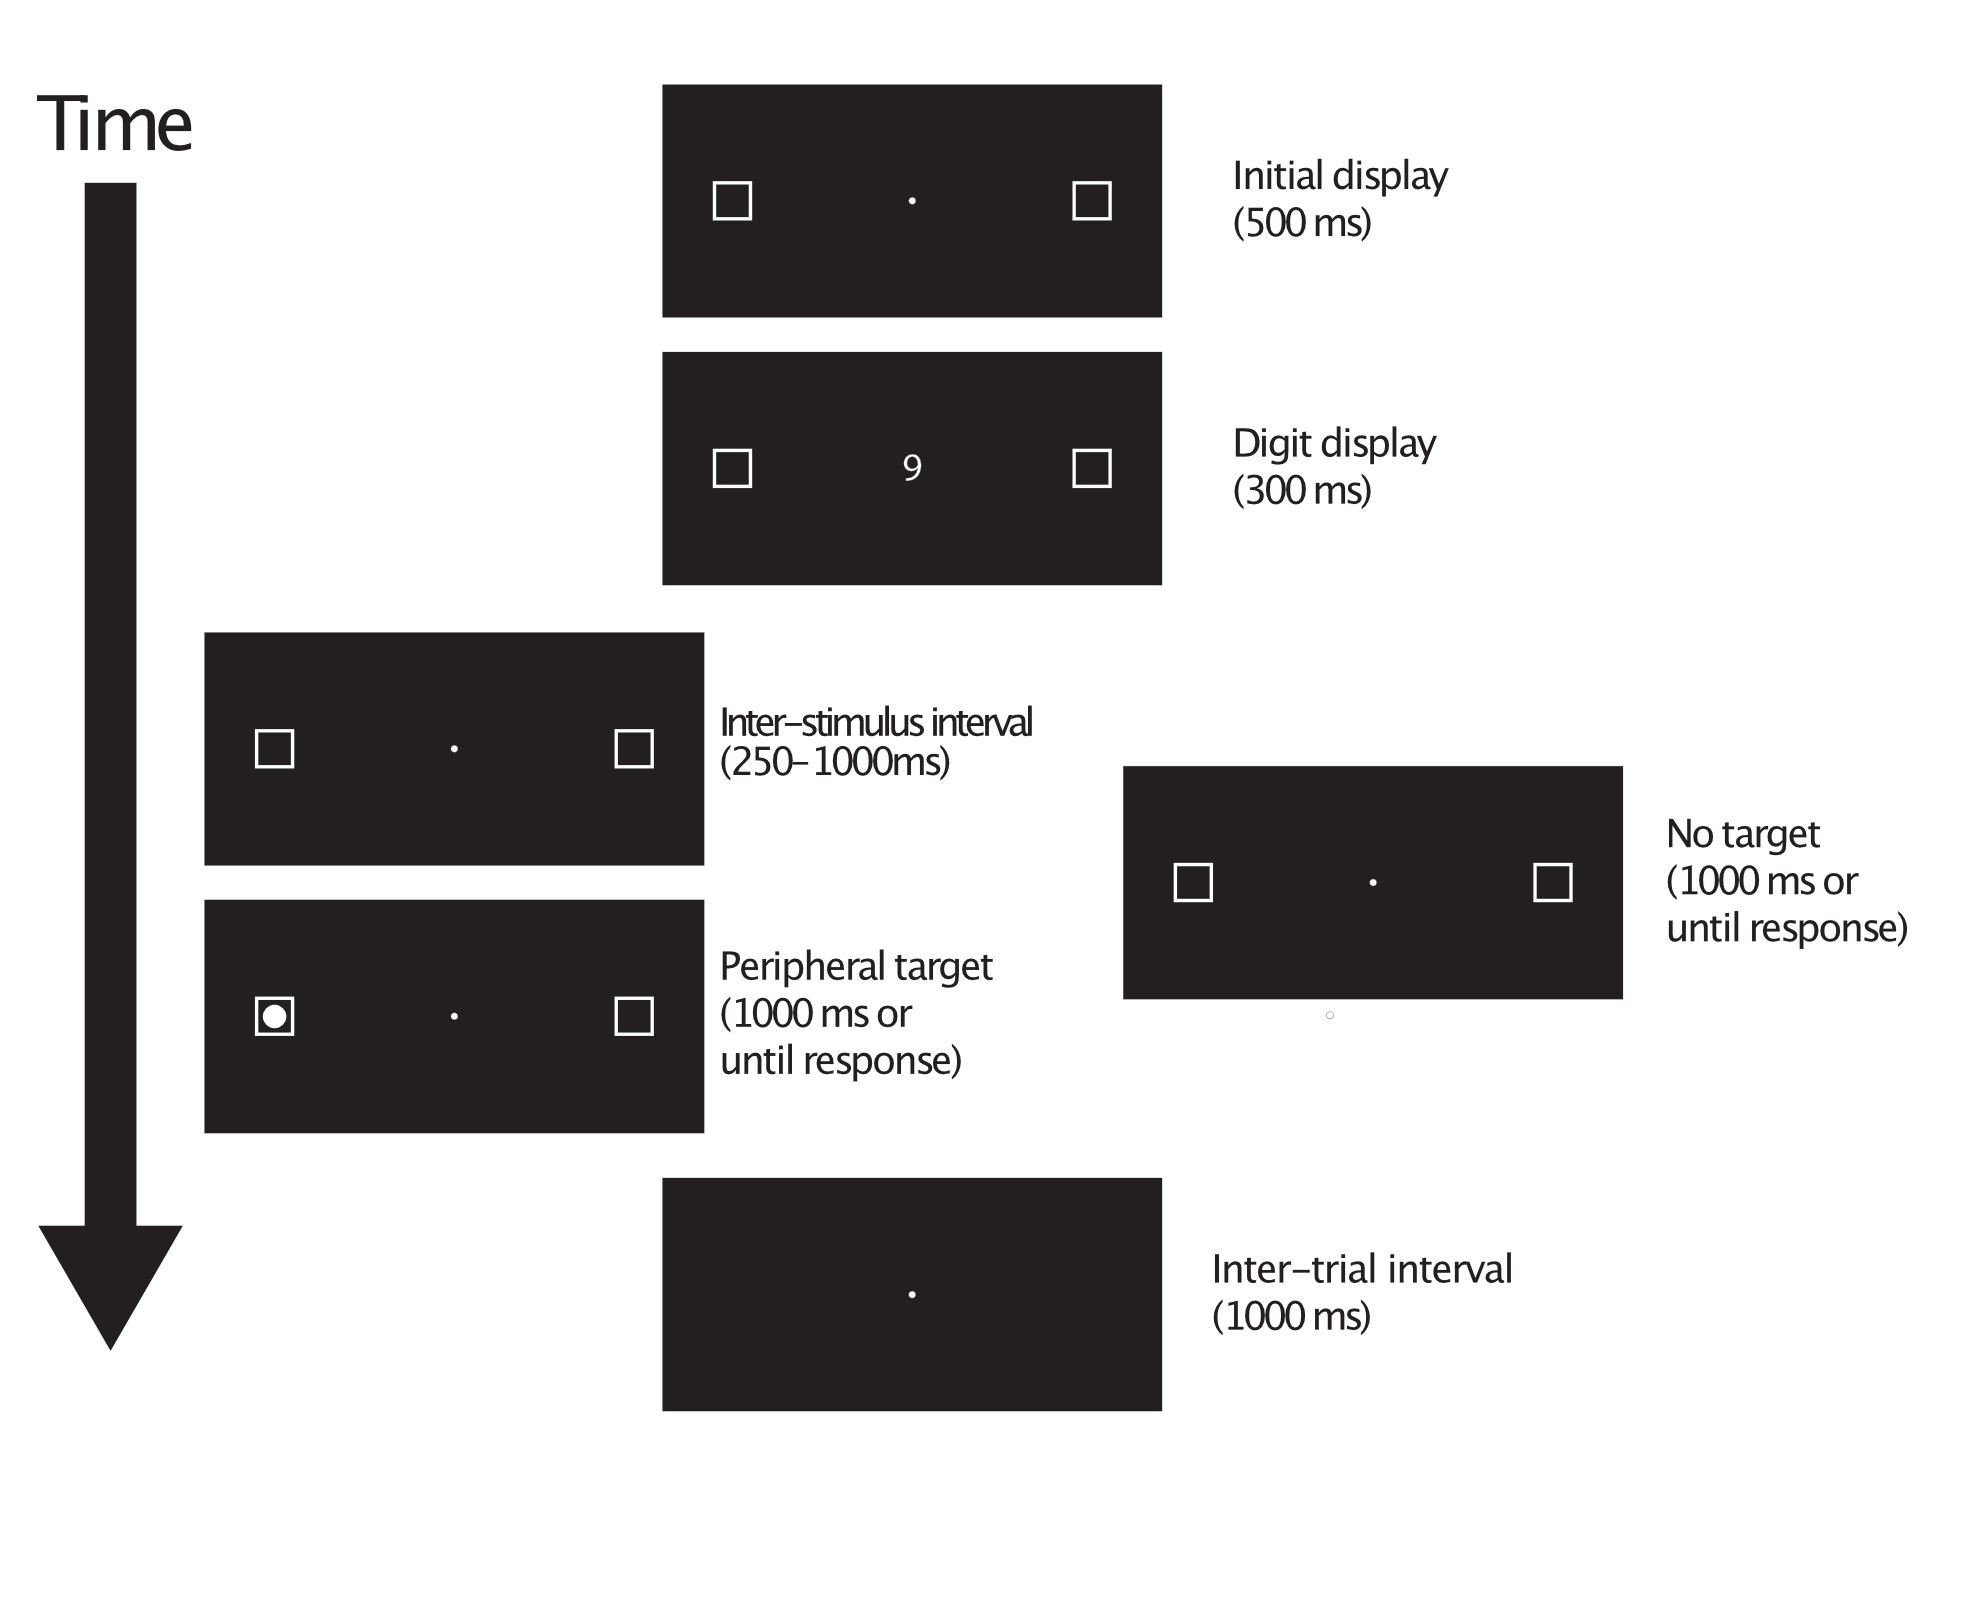
\includegraphics[width=\textwidth]{trialstructure} \caption{Outline of the trial structure for target trials and catch
trials.}\label{fig:Trial}
\end{figure}

\subsection{Eye-tracking protocol}\label{eye-tracking-protocol}

Code implementing an eye-tracking protocol using an EyeLink 1000
eye-tracker was provided to all labs (and is available at
\url{https://github.com/ljcolling/FischerRRR-eyetracking}). For labs
using an eye-tracker other than an EyeLink 1000, deviations from the
standard protocol are listed on the lab-specific OSF page. The standard
nine-point grid was used for calibration and validation at the start of
each block or when required during a block. The start of trials was
triggered after the detection of 500 ms of stable fixation within a 2°
box centred on the fixation point. If the system could not detect a
stable fixation within a 2000 ms time window, the calibration process
was repeated. After the digit was presented, and before the target
appeared, the gaze position was monitored and any deviations outside a
1° box centred on the fixation point were recorded. Any deviations
towards the lateral boxes that exceeded 2° resulted in the trial being
marked as contaminated. These trials were excluded from primary
analyses; however, they were analysed separately to attempt to determine
any possible effect of eye movements on the results.

\subsection{Finger counting}\label{finger-counting}

The finger counting assessment was derived from the task developed by
\textcite{Lucidi:2014gn}. Participants were asked to read aloud four
sentences while counting the number of syllables in each. As reading
aloud prevents prevents participants from verbalising counting, most
participants would need to resort to finger counting while sounding out
the syllables. For each sentence, the experimenter recorded the first
finger and first hand the participant used. While most participants used
their fingers for the task, some participants did not use their fingers
and instead adopted a different strategy. Participant who failed to
engage in finger counting after two sentences were prompted to do so.
Details of the prompting were recorded in lab logs. See OSF for details.

The results of the finger counting task were used to place participants
into one of five groups: left-starters, right-starters, left-prefer,
right-prefer, and no group. The finger counting group was determined not
only by participants' hand preferences but also by how consistently they
engaged in finger counting. The left- (right-)starter group was defined
as those who counted using a hand on all four occasions and used the
left (right) hand on at least three of them. The left (right)-prefer
group was defined as those who counted using a hand on two or three
occasions and used the left (right) hand on at least two of them. The no
group group was defined as all other participants (for example, those
who did not count on their fingers, those who only counted on their
fingers once, and those who counted an equal number of times with each
hand).

\subsection{Reading/writing direction}\label{readingwriting-direction}

Reading and writing direction was determined with a simple three option
questionnaire asking if participants had experience with languages that
are written exclusively from left to right (e.g., English and German),
not exclusively left to right (e.g., Hebrew), or both types (see
\url{https://osf.io/he5za/} for details). This was used to cluster
participants into two groups: exclusively left-to-right readers/writers
and not exclusively left-to-right readers/writers.

\subsection{Handedness}\label{handedness}

To assess handedness, we used the 10-item questionnaire from
\textcite{Nicholls:2013ha}. In labs conducting the experiment in a
language other than English, the questionnaire was translated and some
questions were replaced with more culturally appropriate versions when
required (see \url{https://osf.io/he5za/} for details).

\subsection{Mathematics assessment}\label{mathematics-assessment}

To assess mathematics fluency, we used the short mathematics assessment
employed by \textcite{Tibber:2013ho}. This test is adapted from the
Mathematics Calculation Subtest (WJ-RCalc) of the Woodcock-Johnson III
Tests of Cognitive Abilities \autocite{Woodcock:1989ww}. It contains
twenty-five multiple choice mathematics questions requiring addition,
subtraction, multiplication, and division. Participants had thirty
seconds to select the response on each trial, with the timing controlled
by the computer software. A countdown timer was stationed in the top
left of the screen to inform participants of the time remaining. The
twenty-five questions were split into five levels of five questions. Two
errors on a single level or errors on consecutive levels terminated the
test. The final score was the total number of correct answers.

\subsection{Mathematics anxiety}\label{mathematics-anxiety}

Mathematics anxiety was assessed using the Abbreviated Math Anxiety
Scale \autocite[AMAS;][]{Hopko:2003et}. The AMAS contains nine questions
that ask participants to rate (on a one to five scale) how anxious they
would feel during particular events including thinking of an upcoming
mathematics test, sitting a mathematics examination, and listening to a
mathematics lecture. In labs conducting the experiment in a language
other than English, the AMAS was translated (see
\url{https://osf.io/dhnf8/} for details). The final score was the sum of
the individual ratings, with scores ranging from nine (low anxiety) to
forty-five (high anxiety).

\subsection{Exit questionnaire}\label{exit-questionnaire}

An exit questionnaire that asked participants to describe the purpose of
the experiment was used to determine whether participants could guess
the purpose of the experiment. Participants who correctly guessed the
purpose of the experiment, as judged by the experimenter, were excluded
from primary analyses; however, they were analysed separately to
determine whether this moderated the effect.

\subsection{Exclusion criteria}\label{exclusion-criteria}

Participants whose reaction time data contained more than 5\% catch
trial errors, who correctly guessed the purpose of the experiment or who
who did not undertake all additional assessments were excluded from the
analysis as per our pre-registration plan (see
\url{https://osf.io/6a2ny/}).

\subsection{Analysis}\label{analysis}

The dependent variables of interest were the congruency effect at each
of the four ISI conditions (i.e., 250 ms, 500 ms, 750 ms, and 1000 ms).
This is defined as the average difference in response time between
congruent and incongruent targets, with congruent targets being defined
as left targets preceded by low digits and right targets preceded by
high digits and incongruent targets being defined as left targets
preceded by high digits and right targets preceded by low digits. A
positive value for the congruency effect indicates that participants
were faster at responding to congruent targets relative to incongruent
targets, and a negative value indicates the reverse.

We analysed our data via multilevel multivariate meta-analytic models
\autocite{McSBoc18}. Such models have at least two advantages over the
standard random effects meta-analytic model. First, they better account
for the dependence between our multiple dependent variables (i.e., the
congruency effect at each of the four ISI conditions). Second, rather
than assuming a simple two-level structure, with participants nested
within labs, they can account for more complex nesting structures such
as participants nested within with moderator groups (e.g.,
left-starters, right-starters, etc.) and moderator groups nested within
within labs. In short, the standard approach necessitates treating
several variance components as zero, thereby making unwarranted
independence assumptions.

For each analysis, we consider several simplifications to the equal
allocation multilevel multivariate compound symmetry specification
detailed in \textcite{McSBoc18}; we also consider an equal variance
version of the single correlation equal allocation multilevel
multivariate compound symmetry specification that, using the notation of
that paper, sets the \(\sigma_{d,d}\) equal for all dependent variables
\(d\) (i.e., the congruency effect at each of the four ISI conditions).
We chose among the six specifications via the Akaike Information
Criterion \autocite[AIC;][]{Aki74}.

In analysing the effect of moderators, it would be ideal to consider
them jointly within a single model. However, this would require a
sufficient number of participants in each moderator group. Specifically,
a minimum number of five participants is necessary to compute a 4
\(\times\) 4 covariance matrix of full rank (i.e., corresponding to the
congruency effect at each of the four ISI conditions) as required.
Therefore, the decision on whether to consider all the moderators
jointly within a single model or separately in different models was left
until the sample sizes were known.

Unfortunately, data sparsity prevented us from considering all the
moderators jointly in a single model: when considered jointly, many
combinations of moderators (e.g., finger counting, reading/writing
direction, handedness) result in either zero or very few participants
per moderator group; indeed, this is also the case for some moderators
(i.e., reading/writing direction and handedness) when considered alone
as can be seen in Supplementary Tables \ref{tab:read} and \ref{tab:hand}
respectively. Consequently, we consider each moderator separately
analysing only moderator groups with a minimum of five participants. All
analyses were pre-registered (see \url{https://osf.io/6a2ny/}) and
carried out in accordance with this plan.

For models featuring no moderators (Model 1) or discrete moderators
(finger counting, reading/writing direction, and handedness; Models 2--4
respectively), we analysed the data at the moderator group level as per
\textcite{McSBoc18}. For the model featuring continuous moderators
(mathematics fluency and mathematics anxiety; Model 5), we analysed the
data at the participant level using an analogous specification (see
below for details). Our motivation for considering these moderators and
predictions follow as applicable.

\subsubsection{Model 1: No Moderators}\label{model-1-no-moderators}

\textcite{Fischer:2003ju} suggests a positive congruency effect. The
purpose of Model 1 was to assess this by replicating the analysis
performed by \textcite{Fischer:2003ju}; consequently, it did not account
for any moderators.

\subsubsection{Model 2: Finger counting}\label{model-2-finger-counting}

Recent work suggests that spatial-numerical compatibility effects in
general \autocite{Fischer:2008bv}---including attentional cueing effects
in response to numbers \autocite{Fischer:2014kz}---might be moderated by
finger counting behaviour, specifically being stronger among those who
start finger counting on the left hand and weaker or possibly even
reversed among those who start finger counting on the right hand. The
purpose of Model 2 was to assess this and consequently it took account
of the finger counting moderator.

This model used only data from participants who consistently engaged in
finger counting and consistently started on the same hand, that is,
participants categorised as left-starters or right-starters. We
restricted the analysis to these two groups principally because, if the
finger counting moderator is to have an effect, then we would expect it
to be most prominent in those whose finger counting is clear and
unambiguous.

\subsubsection{Model 3: Reading/writing
direction}\label{model-3-readingwriting-direction}

Recent work suggests that the congruency effect might be weaker or
possibly even reversed among those who have experience with languages
that are not read/written exclusively from left to right
\autocites{Fischer:2008bv}{Shaki:2009ch}. The purpose of Model 3 was to
assess this and consequently it took account of the reading/writing
direction moderator. Specifically, participants were placed into two
groups based on the reading/writing questionnaire: those who read/wrote
exclusively left to right and those who did not.

\subsubsection{Model 4: Handedness}\label{model-4-handedness}

The purpose of Model 4 was to assess whether handedness moderates the
congruency effect and consequently it took account of the handedness
moderator. Specifically, participants were classified as left-handed or
right-handed according to the handedness questionnaire.

\subsubsection{Model 5: Mathematics fluency and mathematics
anxiety}\label{model-5-mathematics-fluency-and-mathematics-anxiety}

Recent work suggests that numerical abilities \autocite{Fischer:2006er}
and mathematics anxiety \autocite{Georges:2016gn} may influence the
strength of spatial-numerical associations. The purpose of Model 5 was
to assess this and consequently it jointly took account of both
mathematics fluency and mathematics anxiety as measured by the maths
test and AMAS respectively.

Specifically, we fit a multilevel model to the participant-level
congruency effects at each of the four ISI conditions; fixed effects
were included for the full set of ISI Condition \(\times\) Maths test
\(\times\) AMAS interactions and random effects were included for (i)
each participant, (ii) each Lab \(\times\) ISI Condition (with equal
variance and zero correlation), and (iii) independently each Lab
\(\times\) Maths test, Lab \(\times\) AMAS, and Lab \(\times\) Maths
test \(\times\) AMAS.

\subsubsection{Secondary analyses}\label{secondary-analyses}

The purpose of our secondary analyses was to assess whether insight into
the purpose of the experiment or eye movements moderate the congruency
effect. Specifically, Model 1 was refit separately to data from
participants who correctly guessed the purpose of the experiment and to
data from eye movement contaminated trials from participants with
contaminated trials at each ISI \(\times\) congruency condition.

\section{Results}\label{results}

\subsection{Replication
operationalisation}\label{replication-operationalisation}

The common definition of replication employed in practice is that a
subsequent study is considered to have successfully replicated a prior
study if either both failed to attain statistical significance or both
attained statistical significance and were directionally consistent.
This definition has been applied analogously in large-scale replication
projects like the present one by comparing the results of a
meta-analysis of the replication studies to the original study in terms
of statistical significance.

However, the null hypothesis significance testing paradigm upon which
this operationalisation of replication is based has been the subject of
no small amount of criticism over the decades \autocites[see, for
example,][]{Rozenboom}{Meehl1978}{Cohen1994}{Gelman2003}{McShane2016}{McShane2017}
and recent calls to abandon it abound
\autocites{Amrhein}{mcshane2019}{Wasserstein}{AmrheinGreendlandMcShane}.
Further, recent work discussing alternative statistical paradigms
specifically in the context of replication \autocite{CollingSzucs} has
called for a better understanding of how statistical inference relates
to scientific inference. A key point is that any assessment of whether a
theory is supported by data depends on whether the magnitude of the
observed effect is consistent with the theory \autocite{Gelman:effect}.
Consequently, in assessing replication, we distinguish between
\emph{statistical hypotheses} and \emph{scientific hypotheses} and focus
on that latter. Specifically, in discussing our results, we do so in
light of the scientific hypothesis advanced by
\textcite{Fischer:2003ju}.

\subsection{Exclusions}\label{exclusions}

In total, seventeen labs contributed data from a total of 1267
participants; 162 were excluded as per our pre-registered criteria
leaving a total of 1105. See Table \ref{tab:Exclusions} for details of
the number of participants collected by each lab, the number analysed,
and the number excluded based on each criterion; the technical error
category includes those participants that were excluded for having
incomplete data due to, for example, equipment failure, experimenter
error, or other technical errors.

\begin{table}[!h]

\caption{\label{tab:Exclusions}Total number of participants, number analysed, number excluded for reasons of technical error, number excluded for more than 5\% catch trial errors, and number excluded for guessing the purpose of the experiment for each lab.}
\centering
\begin{tabular}[t]{lccccc}
\toprule
Lab & \makecell[c]{Total\\Participants} & \makecell[c]{Analysed\\Participants} & \makecell[c]{Technical\\Error} & \makecell[c]{Catch Trial\\Error} & \makecell[c]{Guessed\\Purpose}\\
\midrule
Ansari & 68 & 60 & 2 & 6 & 0\\
Bryce & 68 & 61 & 0 & 3 & 4\\
Chen & 62 & 60 & 1 & 1 & 0\\
Cipora & 93 & 82 & 1 & 3 & 7\\
Colling (Szűcs) & 72 & 65 & 4 & 3 & 0\\
Corballis & 68 & 64 & 2 & 2 & 0\\
Hancock & 66 & 54 & 5 & 6 & 1\\
Holmes & 77 & 60 & 3 & 8 & 6\\
Lindemann & 50 & 47 & 0 & 1 & 2\\
Lukavský & 62 & 61 & 1 & 0 & 0\\
Mammarella & 126 & 103 & 15 & 1 & 7\\
Mieth & 124 & 93 & 2 & 8 & 21\\
Moeller & 77 & 63 & 13 & 1 & 0\\
Ocampo & 60 & 59 & 0 & 0 & 1\\
Ortiz-Ouellet-Lupiáñez-Santiago & 60 & 54 & 3 & 2 & 1\\
Toomarian & 74 & 61 & 4 & 7 & 2\\
Treccani & 60 & 58 & 0 & 1 & 1\\
\bottomrule
\end{tabular}
\end{table}

Five labs used an eye-tracker for at least some of their participants.
See Table \ref{tab:Eyedetail} for details of the number of participants
tested with an eye-tracker, number of participants analysed in our
secondary analysis of eye movement contaminated trials, and number of
eye movement contaminated trials at each ISI \(\times\) congruency
condition for each lab.

\subsection{Preliminary analyses}\label{preliminary-analyses}

Across all 1105 participants and four ISI conditions, the congruency
effect we observed had a mean of 0.24 ms and a standard deviation of
12.48 ms. In addition, across all 1105 participants, it had a mean of
-0.07 ms and a standard deviation of 13.45 ms at the 250 ms ISI
condition, a mean of 0.94 ms and a standard deviation of 12.42 ms at the
500 ms ISI condition, a mean of -0.02 ms and a standard deviation of
12.12 ms at the 750 ms ISI condition, and a mean of 0.10 ms and a
standard deviation of 11.84 ms at the 1000 ms ISI condition. Further,
the correlation between conditions had a mean of 0.00 (and a mean of
0.03 in magnitude) across the six possible pairs of conditions.

In terms of sign, across all 1105 participants and four ISI conditions,
the proportion of times the congruency effect we observed was positive
was 0.50. In addition, across all 1105 participants, this proportion was
0.49 at the 250 ms ISI condition, 0.53 at the 500 ms ISI condition, 0.48
at the 750 ms ISI condition, and 0.50 at the 1000 ms ISI condition.
Further, the proportion of times the number of positive congruency
effects per participant was equal to zero, one, two, three, and four was
respectively 0.06, 0.26, 0.36, 0.26, and 0.06. All of these results are
compatible with the relevant binomial distribution with probability
parameter one-half (i.e., the distribution of the number of heads on
tosses of a fair coin).

\subsection{Primary analyses}\label{primary-analyses}

\subsubsection{Model 1: No moderators}\label{model-1-no-moderators-1}

The purpose of Model 1 was to replicate the analysis performed by
\textcite{Fischer:2003ju}, and thus it did not account for any
moderators. Model 1 was fit to data from 1105 participants from
seventeen labs. We summarise the results from Study 2 of
\textcite{Fischer:2003ju} along with results from each lab and from
Model 1 in Figure \ref{fig:model1}.

The effects we observed both within and across labs were minuscule and
incompatible with those observed in \textcite{Fischer:2003ju}.
Specifically, \textcite{Fischer:2003ju} estimated an effect of -5.00 ms
at the 250 ms ISI condition, 18.00 ms at the 500 ms ISI condition, 23.00
ms at the 750 ms ISI condition, and 11.00 ms at the 1000 ms ISI
condition. In contrast, Model 1 estimates an effect of -0.05 ms, 1.06
ms, 0.19 ms, and 0.18 ms at each of the four respective ISI conditions.

Given this in tandem with the results of our preliminary analyses, we
conclude that we have \emph{failed} to replicate the effect reported by
\textcite{Fischer:2003ju}.

Another major finding was that the effects we observed were highly
consistent not only across ISI conditions but also---perhaps more
surprisingly---across labs. Recent work has found that, contrary to both
substantive and statistical expectations, large-scale replications
projects like the present one tend to show a nontrivial degree of
heterogeneity across labs \autocite{mcshane2019b}. In contrast, we
estimate heterogeneity across labs at 1.02 ms and thus practically
unimportant for most purposes. This suggests that, at least across the
labs involved in the present project, there are unlikely to be lab-level
moderators driving our results. See Table \ref{tab:Exclusions} and
Supplementary Table \ref{tab:mod1} for additional details.

\begin{figure}[H]
    \centering
    \begin{subfigure}{.7\textwidth}
        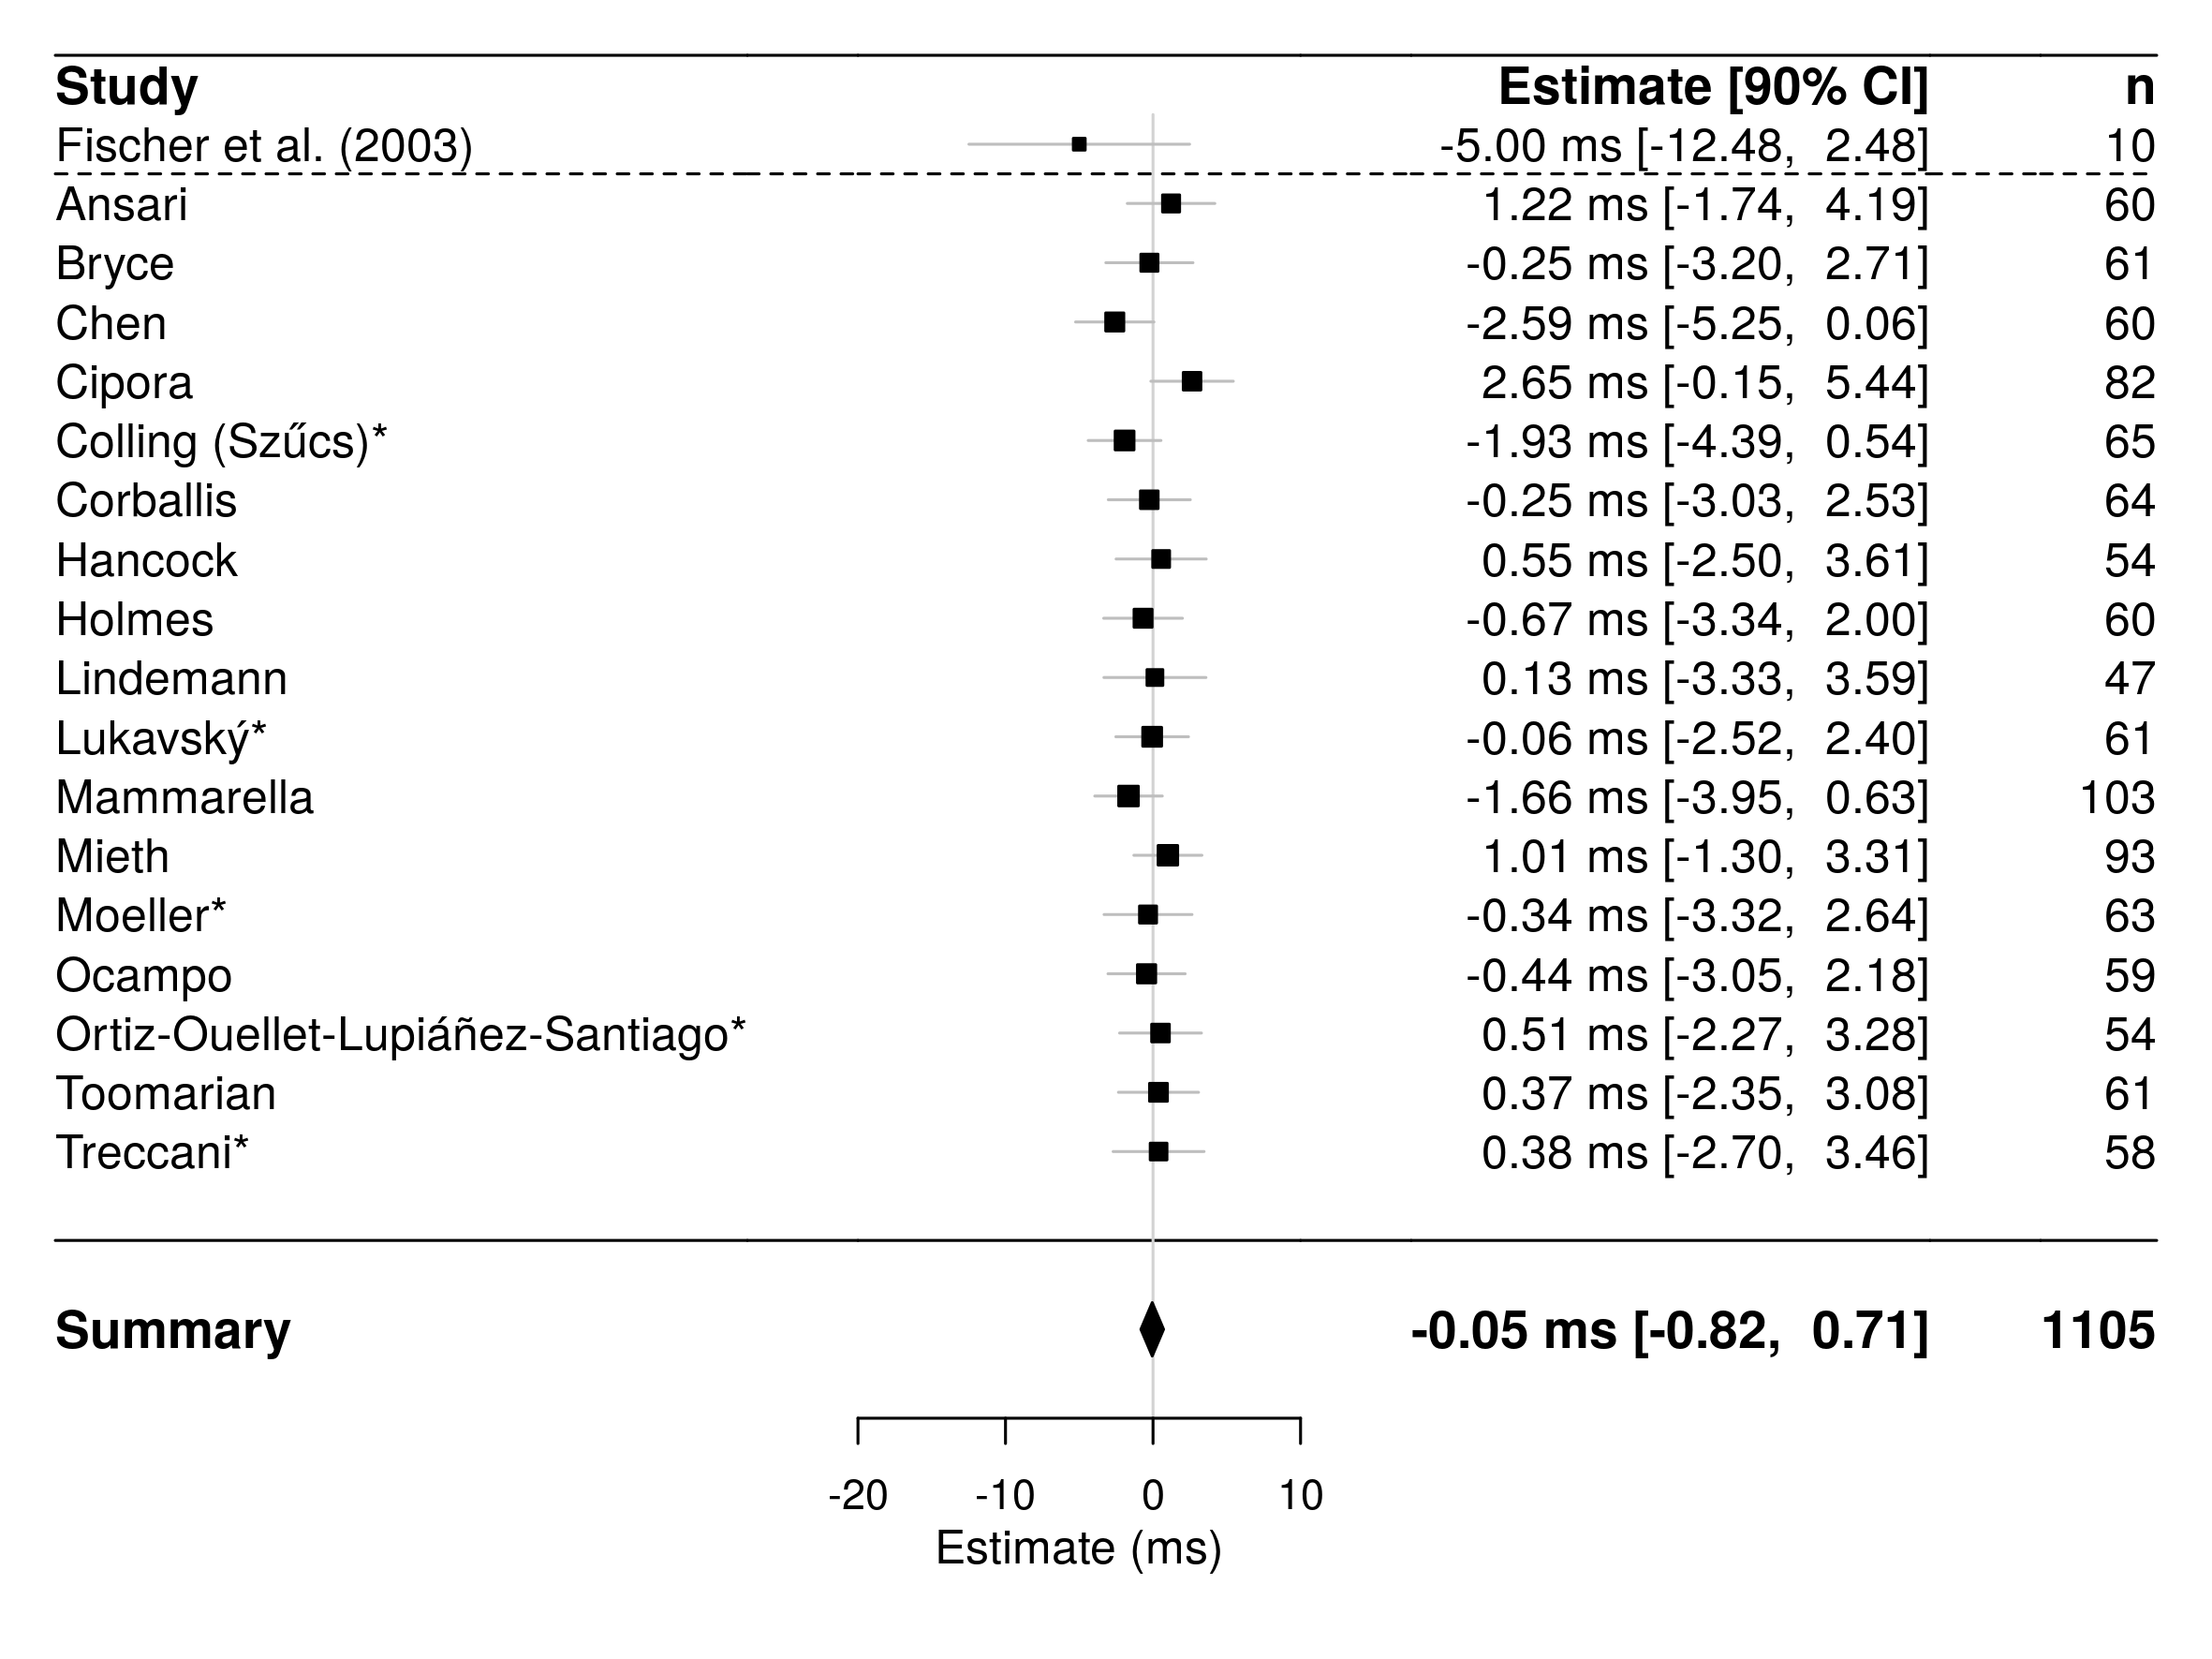
\includegraphics[]{d250}
        \caption{250 ms ISI Condition}
    \end{subfigure}
    \begin{subfigure}{.7\textwidth}
        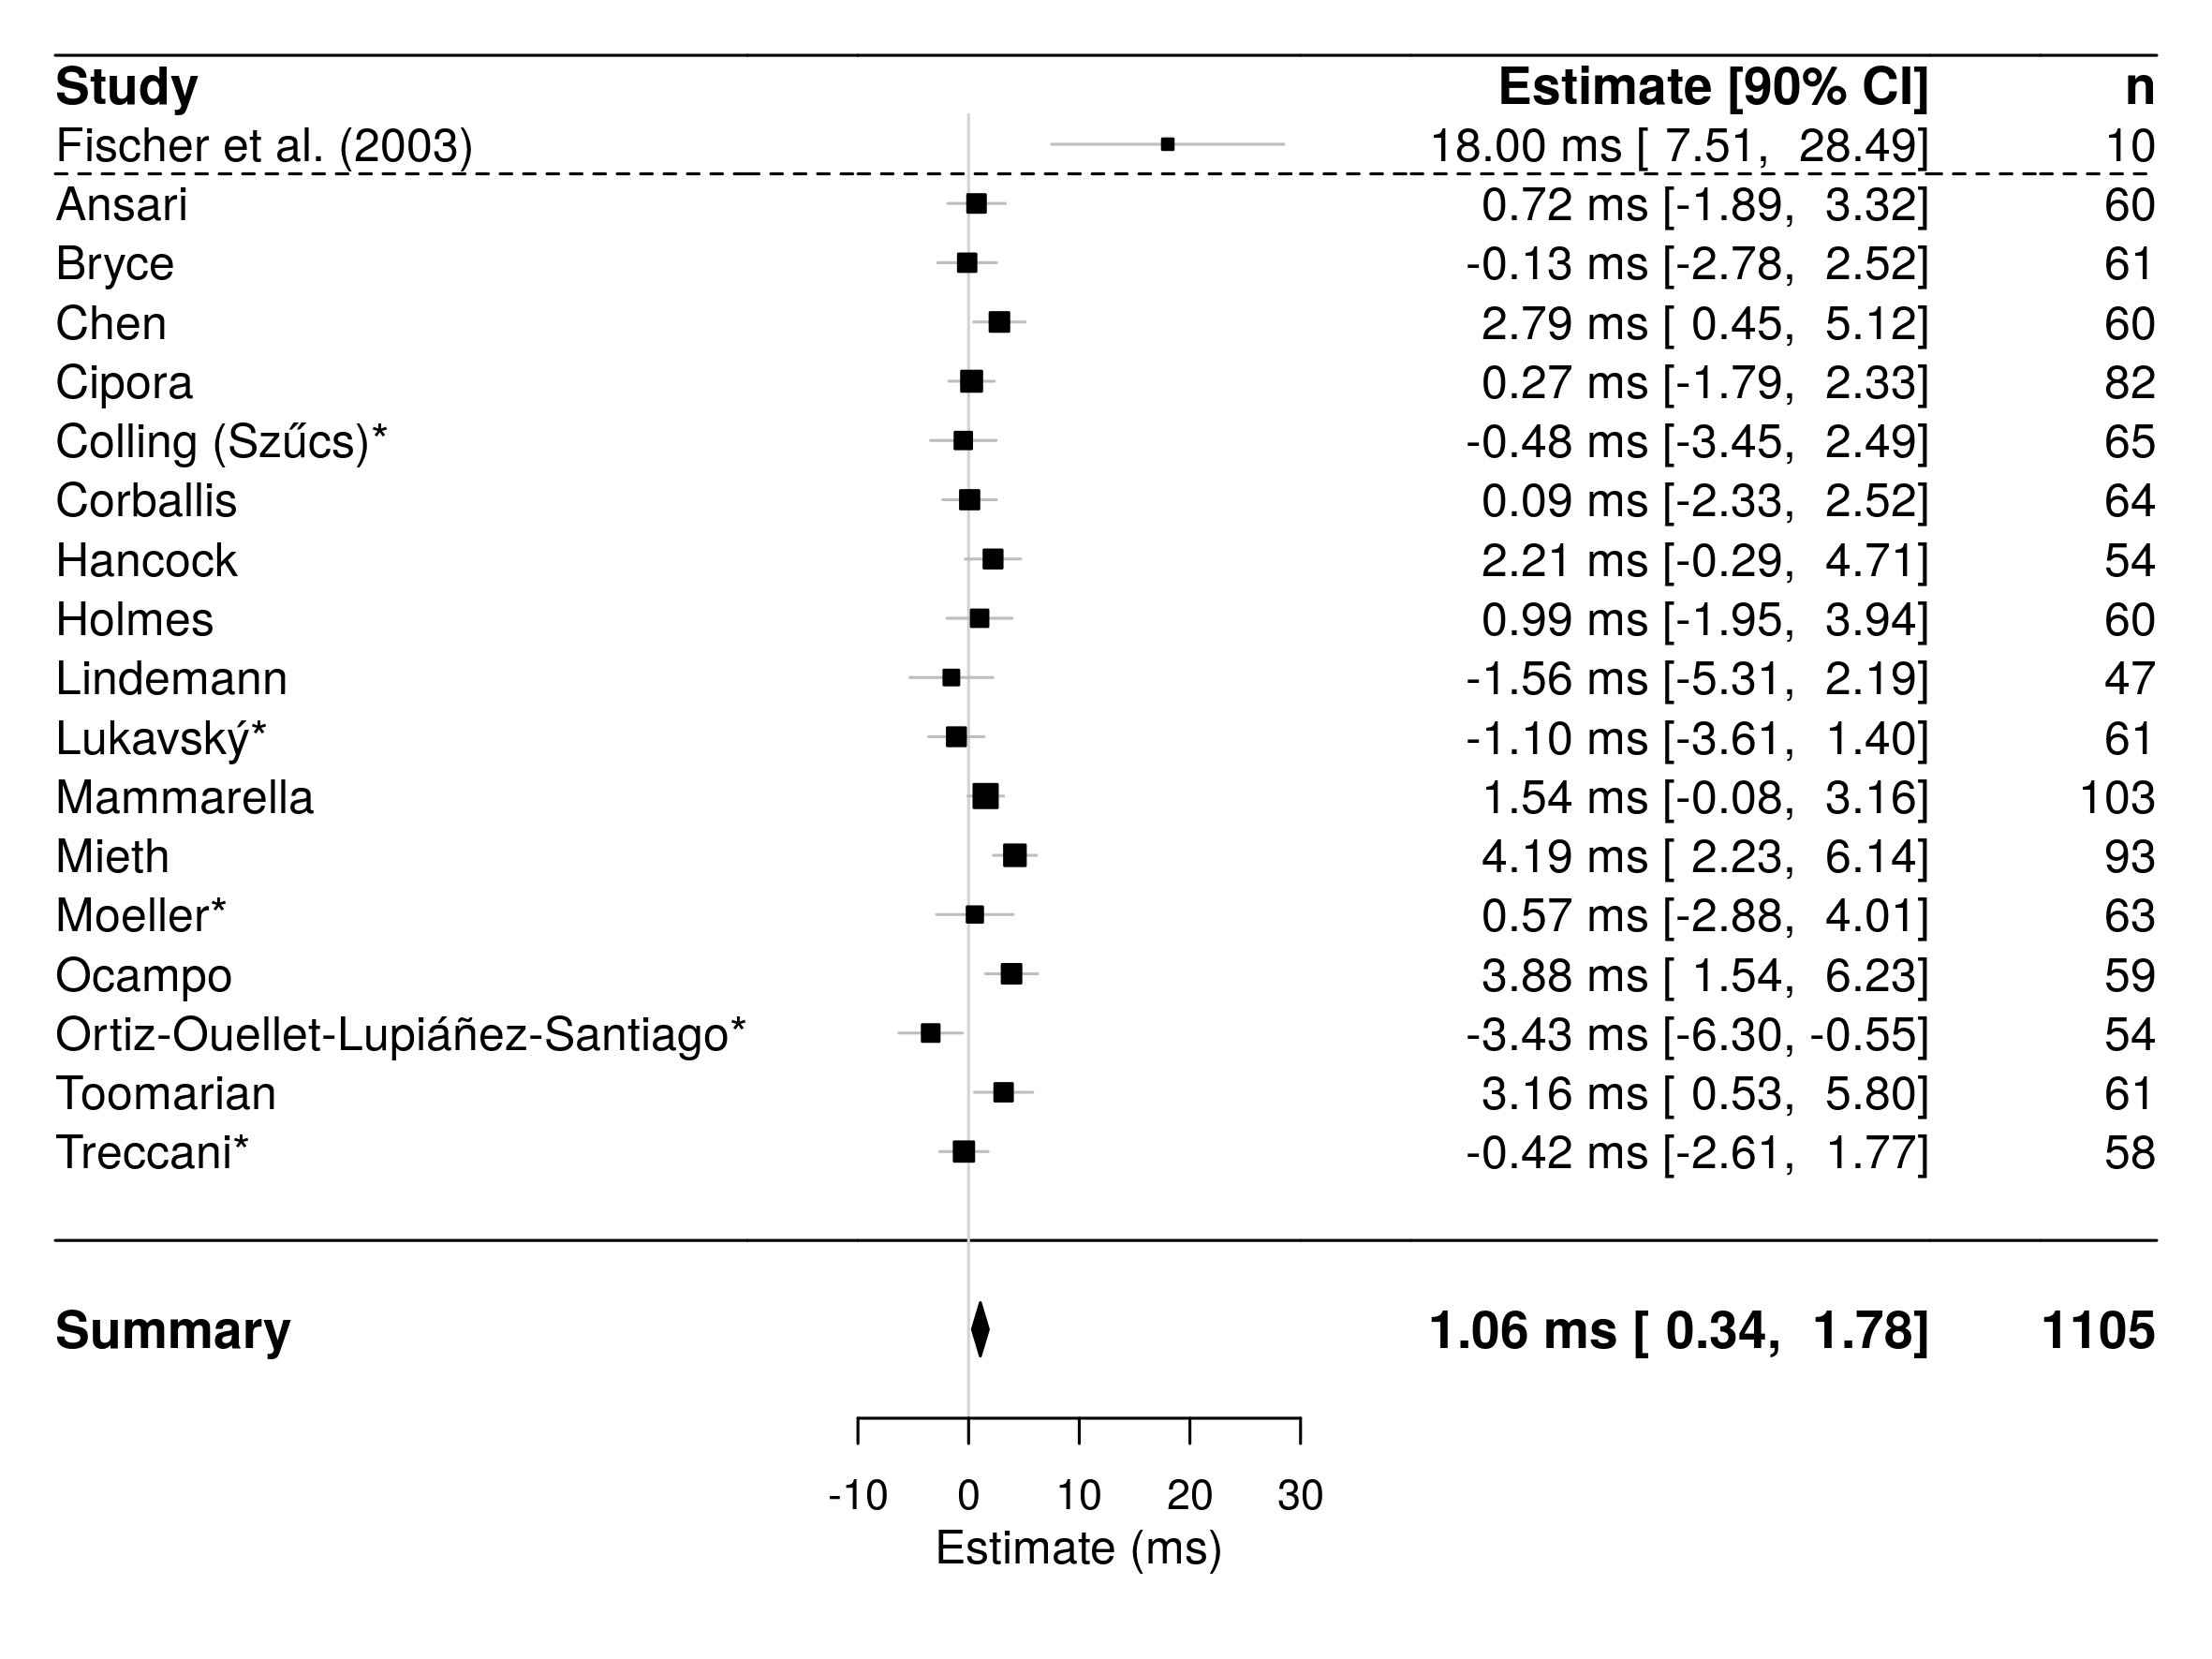
\includegraphics[]{d500}
        \caption{500 ms ISI Condition}
    \end{subfigure}
\end{figure}\begin{figure}[H]
    \centering
    \ContinuedFloat % continue from previous page
    \begin{subfigure}{.7\textwidth}
        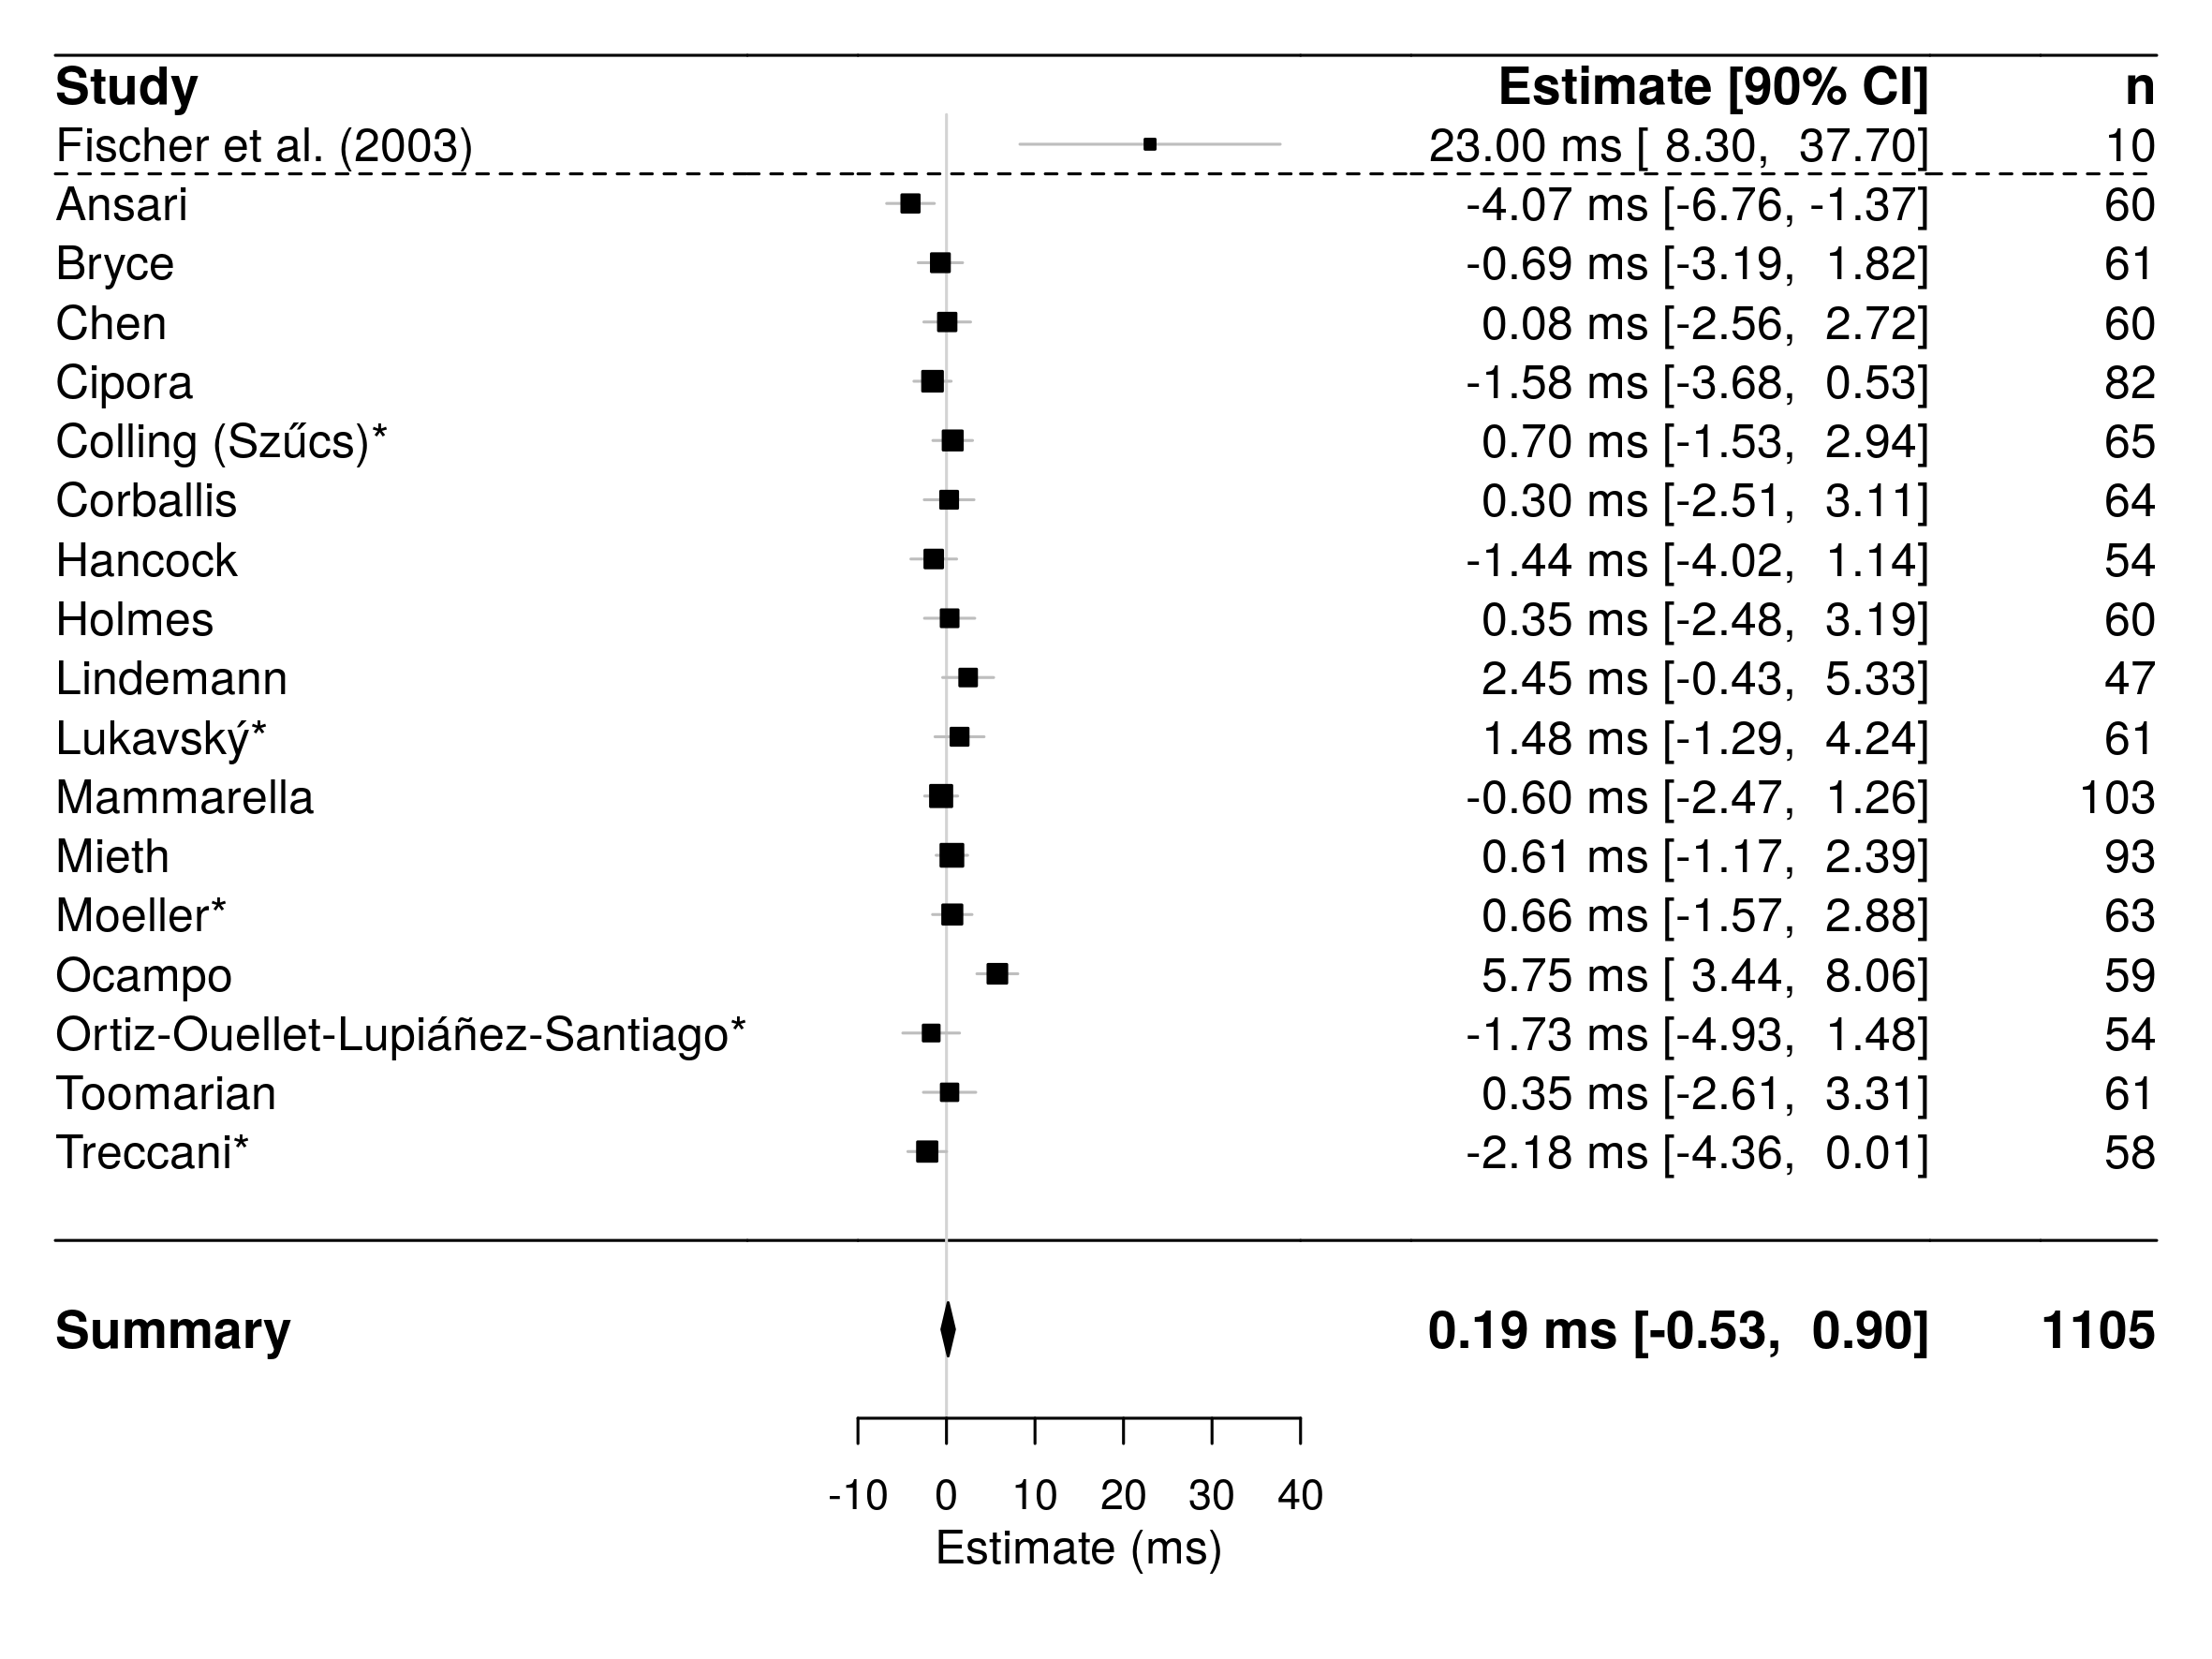
\includegraphics[]{d750}
        \caption{750 ms ISI Condition}
    \end{subfigure}
    \begin{subfigure}{.7\textwidth}
        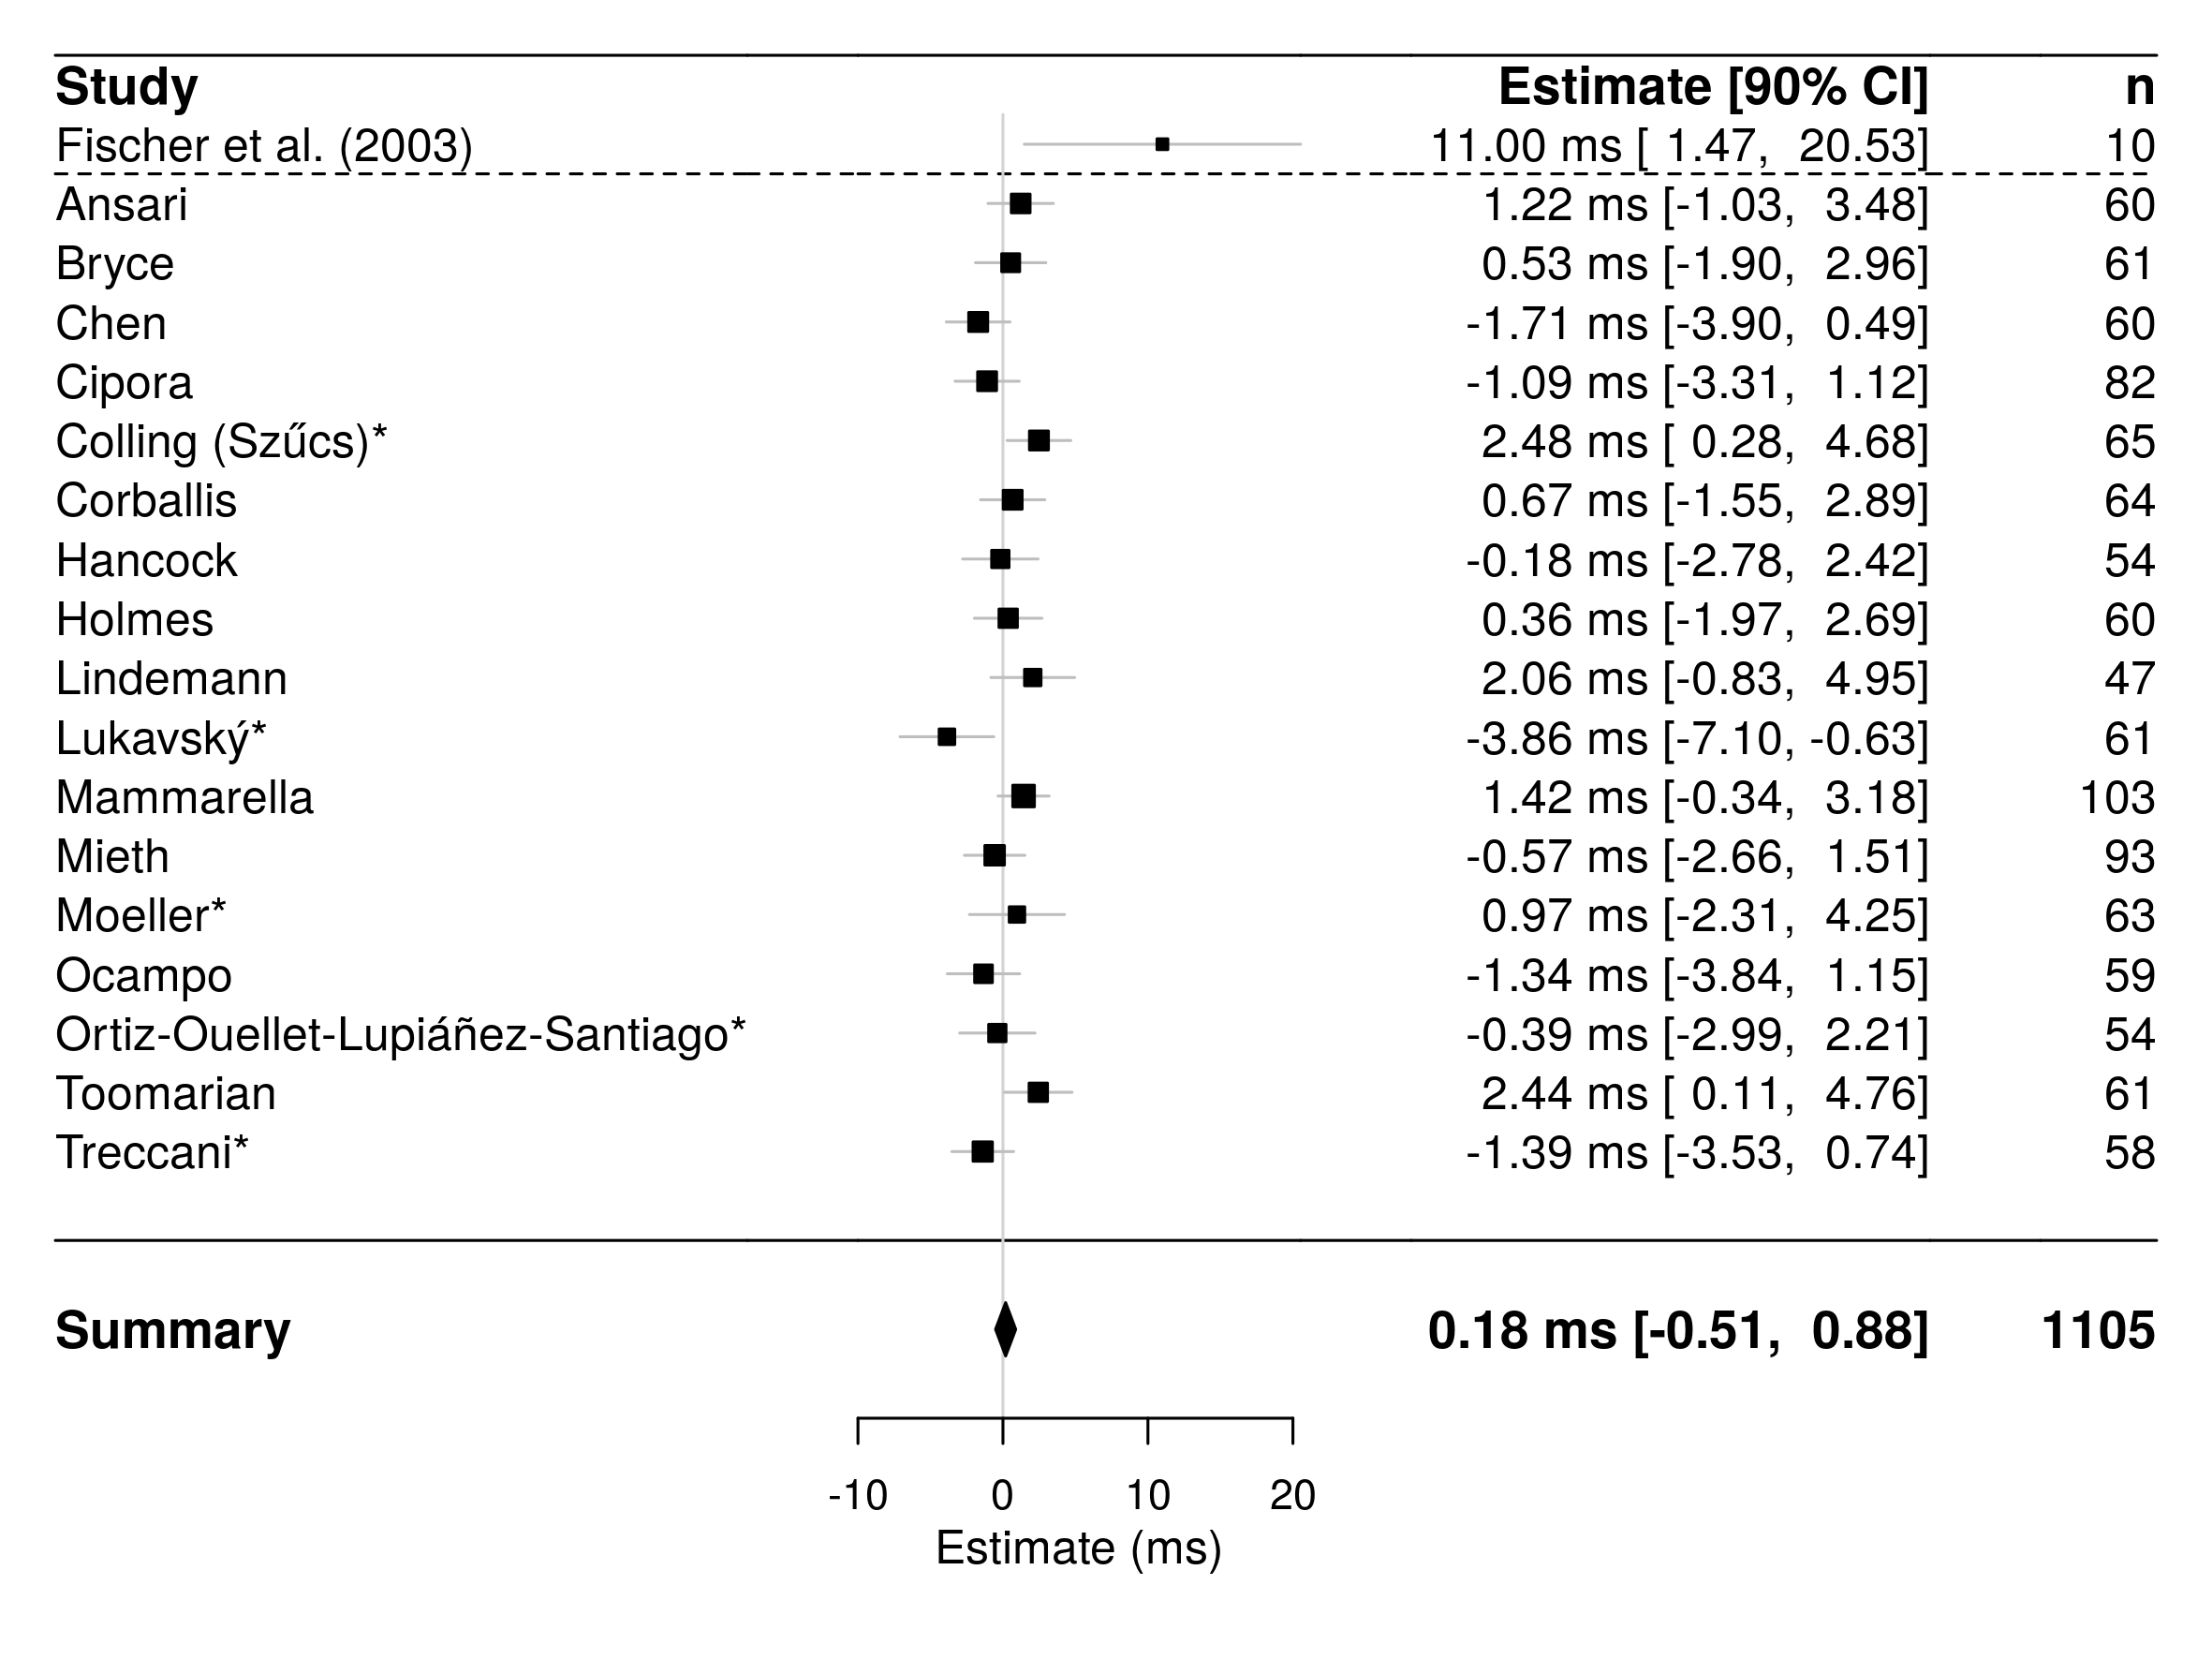
\includegraphics[]{d1000}
        \caption{1000 ms ISI Condition}
    \end{subfigure}
    \caption{Summary of Results from Study 2 of Fischer et al. (2003), Each Lab, and Model 1. The effects we observed both within and across labs were miniscule---around 1 ms---and incompatible with those of around 20 ms observed in Fischer et al. (2003). They were also highly consistent not only across ISI conditions but also---perhaps more surprisingly---across labs with the latter suggesting there are unlikely to be lab-level moderators driving our results Labs using an eye-tracker are marked with an asterisk.}\label{fig:model1}
\end{figure}

\subsubsection{Model 2: Finger
counting}\label{model-2-finger-counting-1}

\begin{figure}
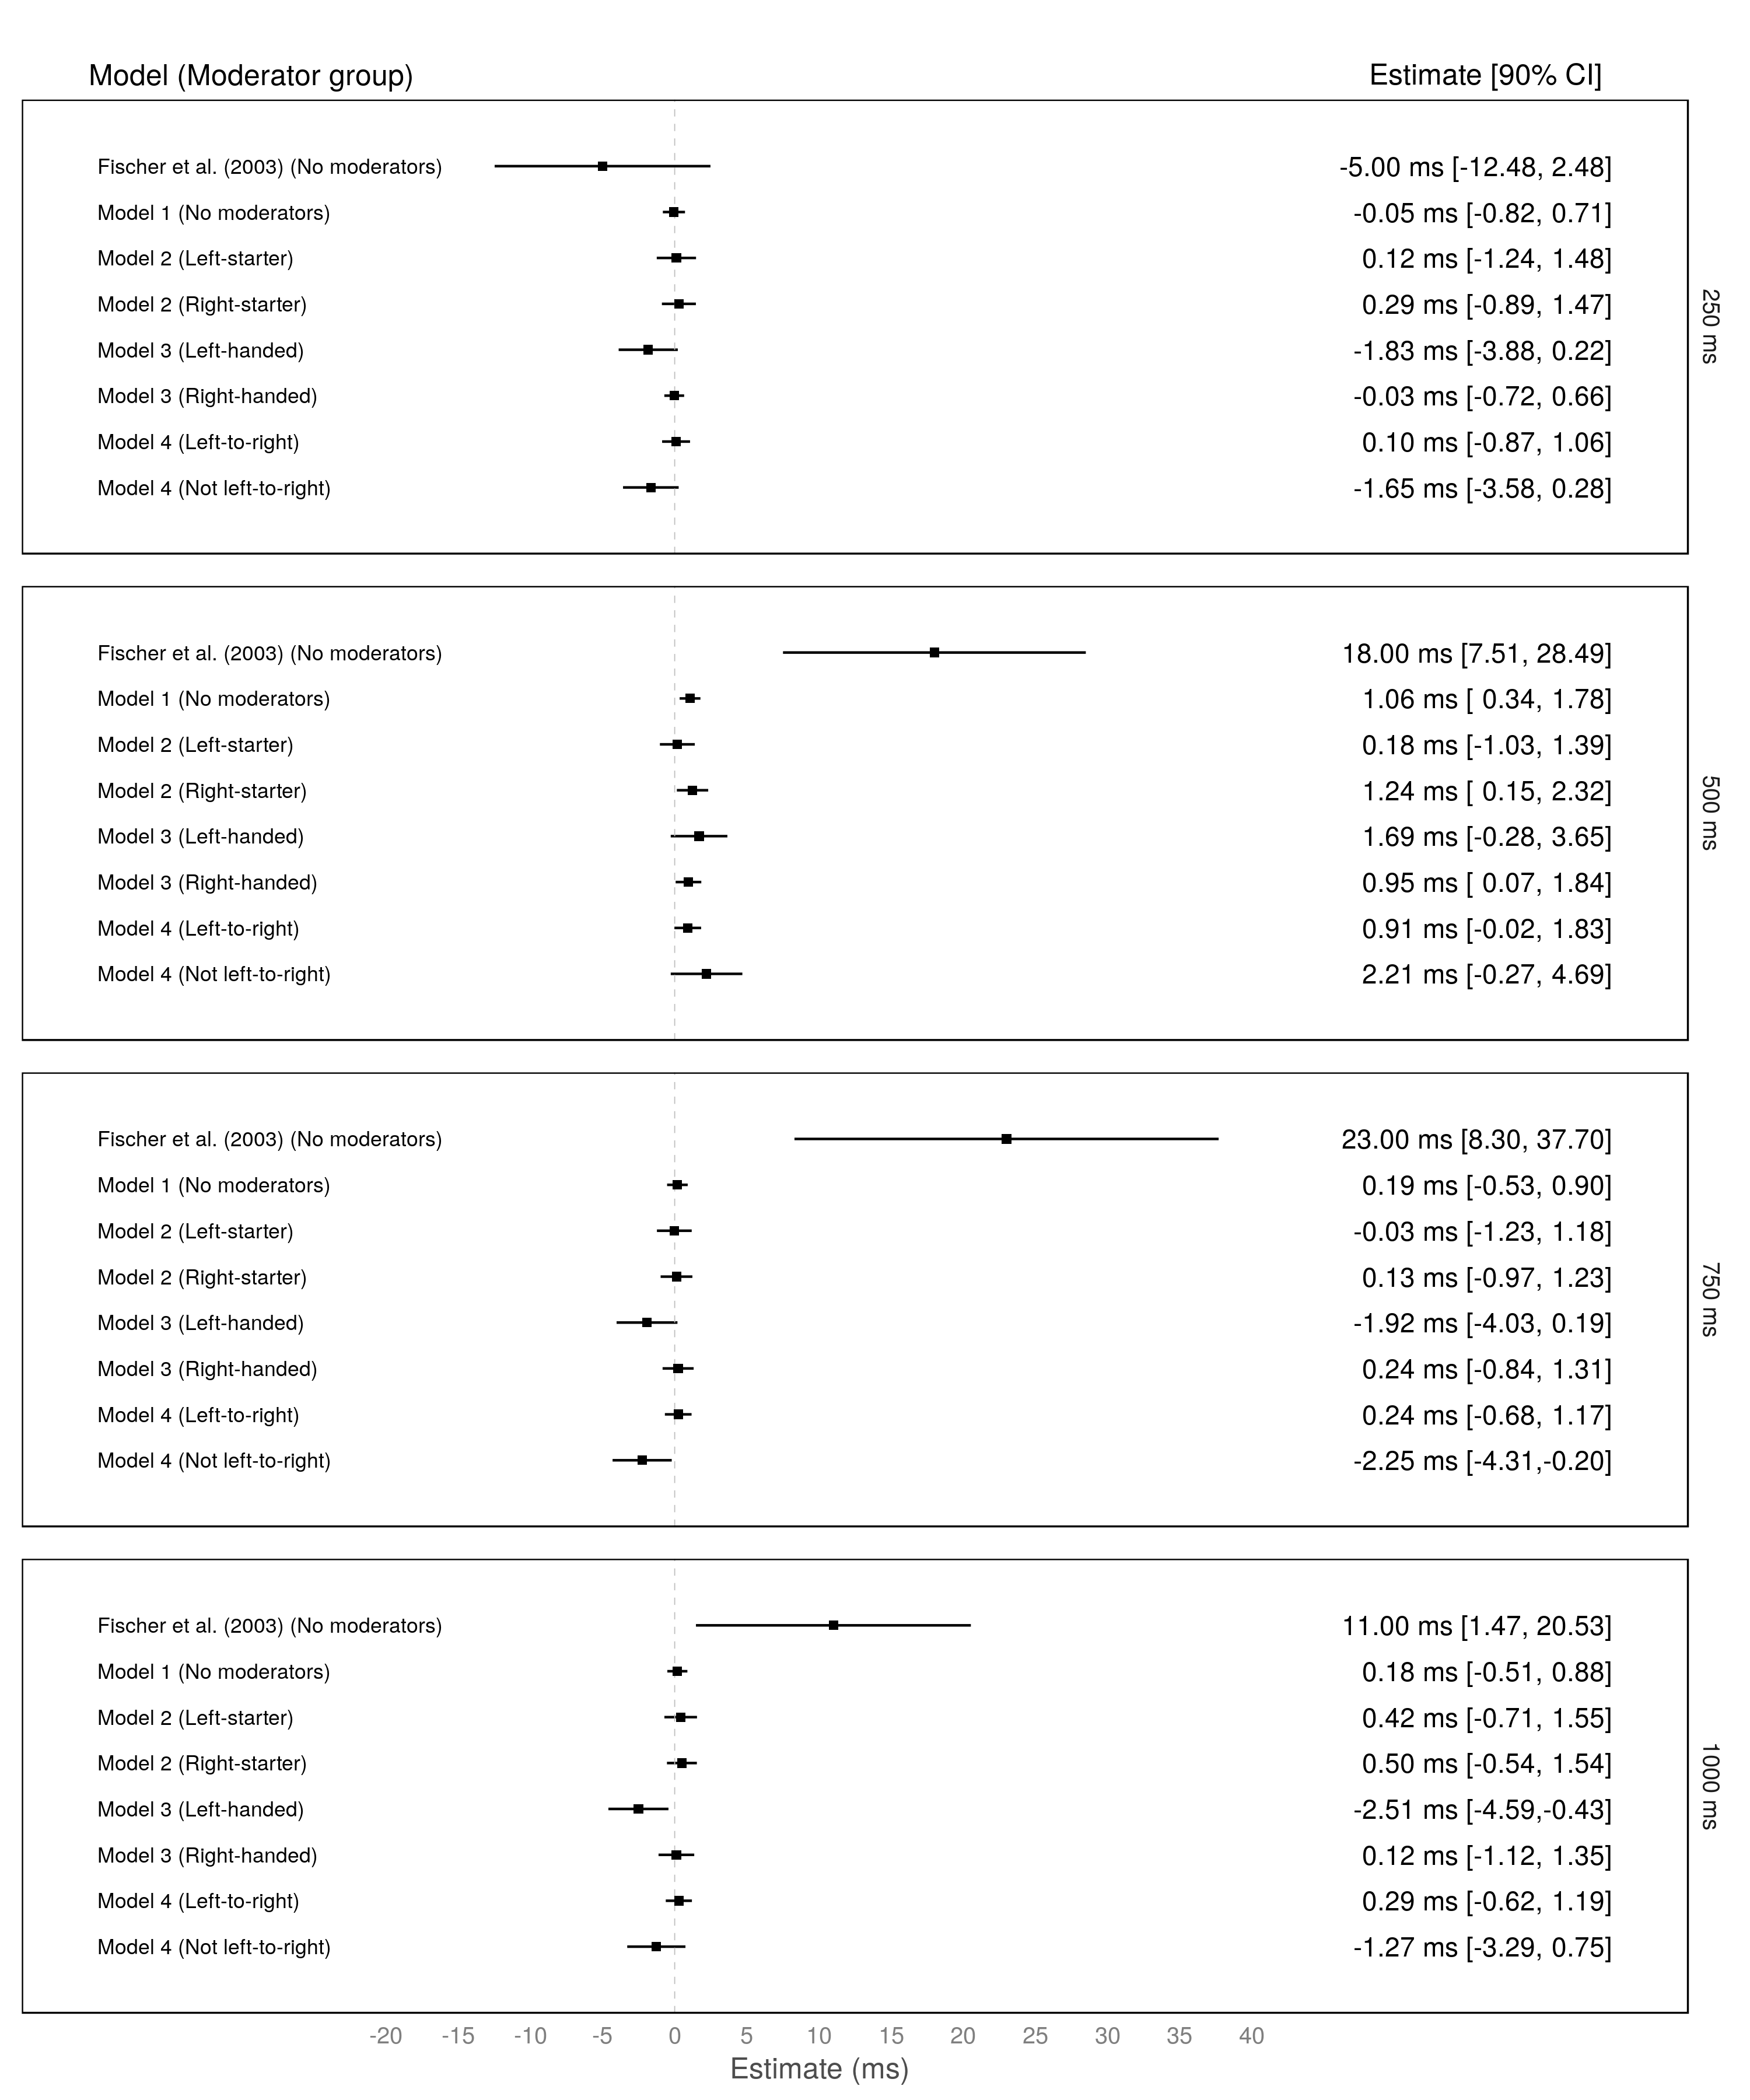
\includegraphics[width=\textwidth]{meta_summaryv4} \caption{Summary of Results from Study 2 of Fischer et al. (2003)
and Models 1--4. The effects we observed were minuscule and incompatible
with those observed in Fischer et al. (2003). They were also highly
consistent across ISI conditions.}\label{fig:metasum}
\end{figure}

Model 2 was fit to data from 343 left-starter participants from
seventeen labs and 482 right-starter participants from seventeen labs.
We summarize the results from Model 2 along with the results from Study
2 of \textcite{Fischer:2003ju} as well as Model 1, Model 3, and Model 4
in Figure \ref{fig:metasum}. While the evidence presented above suggests
a stronger congruency effect among left-starters and a weaker or
possibly even reversed effect among right-starters, as can be seen in
Figure \ref{fig:metasum}, finger counting had no substantial impact on
the results: we observed minuscule effects for each ISI condition and
finger counting group and minuscule differences between the two finger
counting groups at each ISI condition. See Supplementary Table
\ref{tab:count} and Supplementary Table \ref{tab:mod2} for additional
details.






\subsubsection{Model 3: Reading/writing
direction}\label{model-3-readingwriting-direction-1}

Model 3 was fit to data from 1014 exclusively left-to-right
readers/writers from seventeen labs and 76 not exclusively left-to-right
readers/writers from eight labs. While the evidence presented above
suggests a weaker or possibly even reversed congruency effect among
those who have experience with languages that are not read/written
exclusively from left to right, as can be seen in Figure
\ref{fig:metasum}, reading/writing direction had no substantial impact
on the results: we observed minuscule effects for each ISI condition and
reading/writing direction group and minuscule differences between the
two reading/writing direction groups at each ISI condition. See
Supplementary Table \ref{tab:read} and Supplementary Table
\ref{tab:mod3} for additional details.

\subsubsection{Model 4: Handedness}\label{model-4-handedness-1}

Model 4 was fit to data from 69 left-handed participants from nine labs
and 1007 right-handed participants seventeen labs. As can be seen in
Figure \ref{fig:metasum}, handedness had no substantial impact on the
results: we observed minuscule effects for each ISI condition and
handedness group and minuscule differences between the two handedness
groups at each ISI condition. See Supplementary Table \ref{tab:hand} and
Supplementary Table \ref{tab:mod4} for additional details.

\subsubsection{Model 5: Mathematics fluency and mathematics
anxiety}\label{model-5-mathematics-fluency-and-mathematics-anxiety-1}

Model 5 was fit to data from 1105 participants from seventeen labs.
While the evidence presented above suggests mathematics fluency and
mathematics anxiety might moderate congruency effects, we observed no
substantial moderating effects. See Table \ref{tab:Exclusions} and
Supplementary Table \ref{tab:mod5} for additional details.

\subsection{Secondary analyses}\label{secondary-analyses-1}

Model 1 was refit separately to data from 41 participants from four labs
who correctly guessed the purpose of the experiment and to data from
10468 eye movement contaminated trials from 132 participants from five
labs with contaminated trials at each ISI \(\times\) congruency
condition. These analyses yielded nothing of substantive interest. See
Supplementary Materials for details.

\section{Discussion}\label{discussion}

The att-SNARC effect \autocite{Fischer:2003ju} has been used to argue
for an early, response-independent, and automatic origin of the SNARC
effect. If the SNARC effect is produced by early mechanisms, this would
provide good evidence for \enquote{embodied} number representations and
allow for strong claims about the link between number and space (e.g., a
mental number line).

We attempted to replicate Study 2 of \textcite{Fischer:2003ju} by
collecting data from 1105 participants across seventeen labs. Across all
1105 participants and four ISI conditions, the proportion of times the
congruency effect we observed was positive was 0.50. Further, the
effects we observed both within and across labs were miniscule and
incompatible with those observed in \textcite{Fischer:2003ju}. Given
this, we conclude that we have \emph{failed} to replicate the effect
reported by \textcite{Fischer:2003ju}.

The effects we observed were also highly consistent not only across ISI
conditions but also---perhaps more surprisingly---across labs. The
latter suggests there are unlikely to be lab-level moderators driving
our results. In addition, our analysis of several participant-level
moderators (finger counting preferences, reading/writing direction
experience, handedness, and mathematics fluency and mathematics anxiety)
revealed no substantial moderating effects.

We conclude with two important points. First, one might, on the basis of
the common definition of replication employed in practice, object that
we have successfully replicated \textcite{Fischer:2003ju}, at least at
the 500 ms ISI condition. In response, we argue this illustrates one
major flaw of that definition: our result at the 500 ms ISI condition is
manifestly incompatible with the analogous result of
\textcite{Fischer:2003ju}. In addition, we view a difference of about 1
ms, even if \enquote{real}, as too small for any neurally or
psychologically plausible mechanism---particularly one constrained to
operate only within a narrow time window of 500 ms after the digit
display stimulus. That said, we recognize that some such mechanism could
be subject to an arbitrarily large attenuation factor in any particular
experimental paradigm such as that of \textcite{Fischer:2003ju}, and
that potential new paradigms could reveal an effect. Nonetheless, even
were such paradigms forthcoming, we maintain based on these results that
\textcite{Fischer:2003ju} provides no evidence of such a mechanism.

Second, we point to several limitations of the present study. First and
foremost, while our results demonstrate that the att-SNARC effect cannot
be used as evidence to support the strong claims about the link between
number and space discussed above, this does not refute such accounts.
Specifically, while one might, on the basis of our results, prefer
accounts of the SNARC effect that do not imply a mental number line, the
entirety of the evidence for and against different claims about the
SNARC effect must be viewed as a whole. The att-SNARC effect provides
only one such piece of evidence---albeit a particularly strong and
valuable one.

The second set of limitations relates to our sample of subjects. Our
sample was primarily collected from North America, Europe, and
Australasia. Consequently, participants who read/wrote exclusively left
to right are overrepresented in our data. As reading/writing direction
has been shown to strongly moderate spatial-numerical associations, it
would have been preferable to have more participants in this subgroup.
In addition, data sparsity prevented us from considering all the
moderators jointly in a single model and thus we were required to
consider each moderator separately.

Finally, the finger counting assessment we employed did not contain an
explicit instruction to engage in finger counting. As a result, some
participants inconsistently employed finger counting, resulting in them
being excluded from the Model 2 analysis.

\section{Acknowledgements}\label{acknowledgements}

LJC and DS are funded by James S. McDonnell Foundation 21st Century
Science Initiative in Understanding Human Cognition (grant number
220020370; received by DS). We acknowledge the help of the original
authors, in particular Martin Fischer and Jay Pratt. We also note this
project would not have been possible without editor Alex Holcombe's
patient and thoughtful help at every step of the process.

\section{Author contributions}\label{author-contributions}

LJC and DS proposed the study. LJC programmed the experiments. LJC and
BBM conducted the analyses. LJC wrote an initial manuscript. LJC and BBM
wrote revised and final manuscripts. All authors critically reviewed the
final manuscript.

\printbibliography[title=References]

\clearpage
\makeatletter
\efloat@restorefloats
\makeatother


\begin{appendix}
\section{}
\renewcommand{\thetable}{S\arabic{table}}
\renewcommand{\thefigure}{S\arabic{figure}}

\pagenumbering{arabic} \setcounter{page}{1}

\subsection{Primary analyses}\label{primary-analyses}

\subsubsection{Model 1: No Moderators}\label{model-1-no-moderators}

Model 1 was fit to data from 1105 participants from seventeen labs (see
Table \ref{tab:Exclusions} for details). Of the six equal allocation
multilevel multivariate compound symmetry (EAMMCS) model specifications,
the \emph{Equal Variance, Zero Correlation} specification was chosen by
AIC. AIC; fixed effect estimates, standard errors, and \(z\)-statistics;
and variance component estimates are shown in Supplementary Table
\ref{tab:mod1}.

\subsubsection{Model 2: Finger counting}\label{model-2-finger-counting}

Model 2 was fit to data from 343 left-starter participants from
seventeen labs and 482 right-starter participants from seventeen labs
(see Supplementary Table \ref{tab:count} for details). Of the six EAMMCS
model specifications, the \emph{Equal Variance, Zero Correlation}
specification was chosen by AIC. AIC; fixed effect estimates, standard
errors, and \(z\)-statistics; and variance component estimates are shown
in Supplementary Table \ref{tab:mod2}.

\subsubsection{Model 3: Reading/writing
direction}\label{model-3-readingwriting-direction}

Model 3 was fit to data from 1014 exclusively left-to-right
readers/writers from seventeen labs and 76 not exclusively left-to-right
readers/writers from eight labs (see Supplementary Table \ref{tab:read}
for details). Of the six EAMMCS model specifications, the \emph{Equal
Variance, Zero Correlation} specification was chosen by AIC. AIC; fixed
effect estimates, standard errors, and \(z\)-statistics; and variance
component estimates are shown in Supplementary Table \ref{tab:mod3}.

\subsubsection{Model 4: Handedness}\label{model-4-handedness}

Model 4 was fit to data from 69 left-handed participants from nine labs
and 1007 right-handed participants from seventeen labs (see
Supplementary Table \ref{tab:hand} for details). Of the six EAMMCS model
specifications, the \emph{Unequal Variance, Zero Correlation}
specification was chosen by AIC. AIC; fixed effect estimates, standard
errors, and \(z\)-statistics; and variance component estimates are shown
in Supplementary Table \ref{tab:mod4}.

\subsubsection{Model 5: Mathematics fluency and mathematics
anxiety}\label{model-5-mathematics-fluency-and-mathematics-anxiety}

Model 5 was fit to data from 1105 participants from seventeen labs (see
Table \ref{tab:Exclusions}). See the main text for model specification
details, but note that (i) for consistency with Model 1 we employed the
\emph{Equal Variance, Zero Correlation} specification for the Lab
\(\times\) ISI Condition effects and (ii) the maths test and AMAS were
centred and scaled by their respective means and standard deviations
across the 1105 participants prior to estimation of the model. Fixed
effect estimates, standard errors, and \(t\)-statistics and variance
component estimates are shown in Supplementary Table \ref{tab:mod5}.

\subsection{Secondary analyses}\label{secondary-analyses}

\subsubsection{Purpose of experiment}\label{purpose-of-experiment}

Data from several participants were not included in the primary analysis
because they correctly guessed the purpose of the experiment (as
assessed by the exit questionnaire). The data from these participants
was analysed separately to determine whether insight into the purpose of
the experiment moderated the effect. Specifically, Model 1 was refit to
data from the 41 participants from four labs who correctly guessed the
purpose of the experiment (see Supplementary Table \ref{tab:mod1bn} for
details). Of the six model EAMMCS model specifications, the \emph{Equal
Variance, Zero Correlation} specification was chosen by AIC. AIC; fixed
effect estimates, standard errors, and \(z\)-statistics; and variance
component estimates are shown in Supplementary Table \ref{tab:mod1b}.

\subsubsection{Eye-movement contaminated
trials}\label{eye-movement-contaminated-trials}

Data from individual trials that were contaminated with eye movements
were also not included the primary analysis. The data from these trials
was analysed separately to determine whether eye movements moderated the
effect. Specifically, Model 1 was refit to data from 10468 eye movement
contaminated trials from 132 participants from five labs with
contaminated trials at each ISI \(\times\) congruency condition (see
Supplementary Table \ref{tab:Eyedetail} for details). Of the six EAMMCS
model specifications, the \emph{Fixed Effects} specification was chosen
by AIC. AIC; fixed effect estimates, standard errors, and
\(z\)-statistics; and variance component estimates are shown in
Supplementary Table \ref{tab:mod1c}

\begin{table}[!p]
\caption{\label{tab:mod1}Model 1 Estimates.}
\begin{subtable}{\textwidth}
\subcaption{AIC}
\centering
\begin{table}[H]\centering\begingroup\fontsize{10}{12}\selectfont

\begin{tabular}{lr}
\toprule
Specification & AIC\\
\midrule
Fixed Effects & 264.12\\
Equal Variance, Zero Correlation & 259.66\\
Equal Variance, Single Correlation & 261.64\\
Unequal Variance, Zero Correlation & 261.04\\
Unequal Variance, Single Correlation & 260.87\\
No Constraints & 270.83\\
\bottomrule
\end{tabular}\endgroup{}
\end{table}
\end{subtable}
\begin{subtable}{\textwidth}
\caption{Fixed Effect Estimates}
\centering
\begin{table}[H]\centering\begingroup\fontsize{10}{12}\selectfont

\begin{tabular}{lrrr}
\toprule
ISI Condition & Estimate & Std. Err. & $z$\\
\midrule
250  ms & -0.05 & 0.47 & -0.11\\
500  ms & 1.06 & 0.44 & 2.43\\
750  ms & 0.19 & 0.43 & 0.43\\
1000 ms & 0.18 & 0.42 & 0.44\\
\bottomrule
\end{tabular}\endgroup{}
\end{table}
\end{subtable}
\begin{subtable}{\textwidth}
\caption{Variance Component Estimates. Estimates are presented on the standard deviation scale. }
\centering
\begin{table}[H]\centering\begingroup\fontsize{10}{12}\selectfont

\begin{tabular}{lr}
\toprule
ISI Condition & Estimate\\
\midrule
250 ms & 1.02\\
500 ms & 1.02\\
750 ms & 1.02\\
1000 ms & 1.02\\
\bottomrule
\end{tabular}\endgroup{}
\end{table}
\end{subtable}
\end{table}

\begin{table}

\caption{\label{tab:count}Number of participants in each finger counting group for each of the seventeen labs.}
\centering
\begin{tabular}[t]{lccccc}
\toprule
Lab & \makecell[c]{Left-\\Starter} & \makecell[c]{Left-\\Prefer} & \makecell[c]{No\\Group} & \makecell[c]{Right-\\Prefer} & \makecell[c]{Right-\\Starter}\\
\midrule
Ansari & 23 & 2 & 2 & 3 & 30\\
Bryce & 13 & 8 & 2 & 17 & 21\\
Chen & 22 & 0 & 2 & 0 & 36\\
Cipora & 19 & 9 & 5 & 18 & 31\\
Colling (Szűcs) & 21 & 3 & 11 & 3 & 27\\
Corballis & 18 & 3 & 5 & 4 & 34\\
Hancock & 22 & 6 & 0 & 3 & 23\\
Holmes & 14 & 2 & 1 & 8 & 35\\
Lindemann & 22 & 1 & 4 & 1 & 19\\
Lukavský & 12 & 7 & 2 & 16 & 24\\
Mammarella & 30 & 8 & 6 & 23 & 36\\
Mieth & 32 & 10 & 10 & 16 & 25\\
Moeller & 23 & 0 & 6 & 0 & 34\\
Ocampo & 27 & 0 & 2 & 0 & 30\\
Ortiz-Ouellet-Lupiáñez-Santiago & 10 & 8 & 4 & 22 & 10\\
Toomarian & 19 & 0 & 0 & 0 & 42\\
Treccani & 16 & 7 & 4 & 6 & 25\\
\bottomrule
\end{tabular}
\end{table}

\begin{table}[!p]
\caption{\label{tab:mod2}Model 2 Estimates.}
\begin{subtable}{\textwidth}
\subcaption{AIC}
\centering
\begin{table}[H]\centering\begingroup\fontsize{10}{12}\selectfont

\begin{tabular}{lr}
\toprule
Specification & AIC\\
\midrule
Fixed Effects & 665.97\\
Equal Variance, Zero Correlation & 637.31\\
Equal Variance, Single Correlation & 639.00\\
Unequal Variance, Zero Correlation & 638.57\\
Unequal Variance, Single Correlation & 640.13\\
No Constraints & 646.51\\
\bottomrule
\end{tabular}\endgroup{}
\end{table}
\end{subtable}
\begin{subtable}{\textwidth}
\caption{Fixed Effect Estimates}
\centering
\begin{table}[H]\centering\begingroup\fontsize{10}{12}\selectfont

\begin{tabular}{llrrr}
\toprule
ISI Condition & Finger counting group & Estimate & Std. Err. & $z$\\
\midrule
250  ms & Right-starter & 0.29 & 0.72 & 0.40\\
250  ms & Left-starter & 0.12 & 0.83 & 0.14\\
500  ms & Right-starter & 1.24 & 0.66 & 1.88\\
500  ms & Left-starter & 0.18 & 0.74 & 0.24\\
750  ms & Right-starter & 0.13 & 0.67 & 0.19\\
750  ms & Left-starter & -0.03 & 0.73 & -0.04\\
1000 ms & Right-starter & 0.50 & 0.63 & 0.79\\
1000 ms & Left-starter & 0.42 & 0.69 & 0.61\\
\bottomrule
\end{tabular}\endgroup{}
\end{table}
\end{subtable}
\begin{subtable}{\textwidth}
\caption{Variance Component Estimates. Estimates are presented on the standard deviation scale. 39\% of the variance is estimated to be at the lab-level and 61\% at the group-level.}
\centering
\begin{table}[H]\centering\begingroup\fontsize{10}{12}\selectfont

\begin{tabular}{lr}
\toprule
ISI Condition & Estimate\\
\midrule
250 ms & 1.74\\
500 ms & 1.74\\
750 ms & 1.74\\
1000 ms & 1.74\\
\bottomrule
\end{tabular}\endgroup{}
\end{table}
\end{subtable}
\end{table}

\begin{table}

\caption{\label{tab:read}Number of participants in each of the reading/writing direction groups for each of the seventeen labs.}
\centering
\begin{tabular}[t]{lcc}
\toprule
Lab & \makecell[c]{Exclusively\\Left-to-Right} & \makecell[c]{Not exclusively\\Left-to-Right}\\
\midrule
Ansari & 55 & 5\\
Bryce & 59 & 2\\
Chen & 39 & 21\\
Cipora & 76 & 6\\
Colling (Szűcs) & 55 & 10\\
Corballis & 60 & 4\\
Hancock & 53 & 1\\
Holmes & 54 & 6\\
Lindemann & 47 & 0\\
Lukavský & 58 & 3\\
Mammarella & 103 & 0\\
Mieth & 79 & 14\\
Moeller & 54 & 9\\
Ocampo & 55 & 4\\
Ortiz-Ouellet-Lupiáñez-Santiago & 54 & 0\\
Toomarian & 56 & 5\\
Treccani & 57 & 1\\
\bottomrule
\end{tabular}
\end{table}

\begin{table}[!p]
\caption{\label{tab:mod3}Model 3 Estimates.}
\begin{subtable}{\textwidth}
\subcaption{AIC}
\centering
\begin{table}[H]\centering\begingroup\fontsize{10}{12}\selectfont

\begin{tabular}{lr}
\toprule
Specification & AIC\\
\midrule
Fixed Effects & 495.58\\
Equal Variance, Zero Correlation & 448.05\\
Equal Variance, Single Correlation & 449.41\\
Unequal Variance, Zero Correlation & 451.89\\
Unequal Variance, Single Correlation & 453.44\\
No Constraints & 457.83\\
\bottomrule
\end{tabular}\endgroup{}
\end{table}
\end{subtable}
\begin{subtable}{\textwidth}
\caption{Fixed Effect Estimates}
\centering
\begin{table}[H]\centering\begingroup\fontsize{10}{12}\selectfont

\begin{tabular}{llrrr}
\toprule
ISI Condition &  Reading/Writing Direction & Estimate & Std. Err. & $z$\\
\midrule
250  ms & Exclusively LTR & 0.10 & 0.59 & 0.17\\
250  ms & Not exclusively LTR & -1.65 & 1.17 & -1.41\\
500  ms & Exclusively LTR & 0.91 & 0.56 & 1.62\\
500  ms & Not exclusively LTR & 2.21 & 1.51 & 1.46\\
750  ms & Exclusively LTR & 0.24 & 0.56 & 0.43\\
750  ms & Not exclusively LTR & -2.25 & 1.25 & -1.80\\
1000 ms & Exclusively LTR & 0.29 & 0.55 & 0.53\\
1000 ms & Not exclusively LTR & -1.27 & 1.23 & -1.03\\
\bottomrule
\end{tabular}\endgroup{}
\end{table}
\end{subtable}
\begin{subtable}{\textwidth}
\caption{Variance Component Estimates. Estimates are presented on the standard deviation scale. 10\% of the variance is estimated to be at the lab-level and 90\% at the group-level.}
\centering
\begin{table}[H]\centering\begingroup\fontsize{10}{12}\selectfont

\begin{tabular}{lr}
\toprule
ISI Condition & Estimate\\
\midrule
250 ms & 1.71\\
500 ms & 1.71\\
750 ms & 1.71\\
1000 ms & 1.71\\
\bottomrule
\end{tabular}\endgroup{}
\end{table}
\end{subtable}
\end{table}

\begin{table}

\caption{\label{tab:hand}Number of participants in each handedness group for each of the seventeen labs.}
\centering
\begin{tabular}[t]{lcc}
\toprule
Lab & \makecell[c]{Left-\\handed} & \makecell[c]{Right-\\handed}\\
\midrule
Ansari & 4 & 56\\
Bryce & 4 & 57\\
Chen & 5 & 55\\
Cipora & 3 & 79\\
Colling (Szűcs) & 7 & 58\\
Corballis & 9 & 55\\
Hancock & 6 & 48\\
Holmes & 4 & 56\\
Lindemann & 5 & 42\\
Lukavský & 7 & 54\\
Mammarella & 6 & 97\\
Mieth & 14 & 79\\
Moeller & 4 & 59\\
Ocampo & 4 & 55\\
Ortiz-Ouellet-Lupiáñez-Santiago & 3 & 51\\
Toomarian & 10 & 51\\
Treccani & 3 & 55\\
\bottomrule
\end{tabular}
\end{table}

\begin{table}[!p]
\caption{\label{tab:mod4}Model 4 Estimates.}
\begin{subtable}{\textwidth}
\subcaption{AIC}
\centering
\begin{table}[H]\centering\begingroup\fontsize{10}{12}\selectfont

\begin{tabular}{lr}
\toprule
Specification & AIC\\
\midrule
Fixed Effects & 598.41\\
Equal Variance, Zero Correlation & 473.56\\
Equal Variance, Single Correlation & 475.56\\
Unequal Variance, Zero Correlation & 470.86\\
Unequal Variance, Single Correlation & 472.48\\
No Constraints & 480.12\\
\bottomrule
\end{tabular}\endgroup{}
\end{table}
\end{subtable}
\begin{subtable}{\textwidth}
\caption{Fixed Effect Estimates}
\centering
\begin{table}[H]\centering\begingroup\fontsize{10}{12}\selectfont

\begin{tabular}{llrrr}
\toprule
ISI Condition & Handedness Group & Estimate & Std. Err. & $z$\\
\midrule
250  ms & Right-handed & -0.03 & 0.42 & -0.07\\
250  ms & Left-handed & -1.83 & 1.25 & -1.46\\
500  ms & Right-handed & 0.95 & 0.54 & 1.76\\
500  ms & Left-handed & 1.69 & 1.19 & 1.42\\
750  ms & Right-handed & 0.24 & 0.65 & 0.37\\
750  ms & Left-handed & -1.92 & 1.28 & -1.50\\
1000 ms & Right-handed & 0.12 & 0.75 & 0.16\\
1000 ms & Left-handed & -2.51 & 1.27 & -1.98\\
\bottomrule
\end{tabular}\endgroup{}
\end{table}
\end{subtable}
\begin{subtable}{\textwidth}
\caption{Variance Component Estimates. Estimates are presented on the standard deviation scale. 12\% of the variance is estimated to be at the lab-level and 88\% at the group-level.}
\centering
\begin{table}[H]\centering\begingroup\fontsize{10}{12}\selectfont

\begin{tabular}{lr}
\toprule
ISI Condition & Estimate\\
\midrule
250 ms & 0.01\\
500 ms & 1.57\\
750 ms & 2.19\\
1000 ms & 2.71\\
\bottomrule
\end{tabular}\endgroup{}
\end{table}
\end{subtable}
\end{table}

\begin{table}[!p]
\caption{\label{tab:mod5}Model 5 Estimates.}
\begin{subtable}{\textwidth}
\subcaption{Fixed Effect Estimates}
\centering
\begin{table}[H]\centering\begingroup\fontsize{10}{12}\selectfont

\begin{tabular}{lccc}
\toprule
Effect & Estimate & Std. Err. & $t$\\
\midrule
250 ms ISI & -0.03 & 0.44 & -0.07\\
500 ms ISI & 0.88 & 0.44 & 2.02\\
750 ms ISI & 0.01 & 0.44 & 0.02\\
1000 ms ISI & 0.21 & 0.44 & 0.48\\
250 ms ISI $\times$ Maths test & -0.15 & 0.42 & -0.35\\
500 ms ISI $\times$ Maths test & -0.80 & 0.42 & -1.90\\
750 ms ISI $\times$ Maths test & -0.24 & 0.42 & -0.57\\
1000 ms ISI $\times$ Maths test & 0.08 & 0.42 & 0.18\\
250 ms ISI $\times$ AMAS & -0.66 & 0.40 & -1.66\\
500 ms ISI $\times$ AMAS & 0.29 & 0.40 & 0.73\\
750 ms ISI $\times$ AMAS & -0.21 & 0.40 & -0.54\\
1000 ms ISI $\times$ AMAS & -0.57 & 0.40 & -1.44\\
250 ms ISI $\times$ Maths test $\times$ AMAS & -0.12 & 0.39 & -0.30\\
500 ms ISI $\times$ Maths test $\times$ AMAS & -0.38 & 0.39 & -0.98\\
750 ms ISI $\times$ Maths test $\times$ AMAS & -0.24 & 0.39 & -0.63\\
1000 ms ISI $\times$ Maths test $\times$ AMAS & 0.22 & 0.39 & 0.56\\
\bottomrule
\end{tabular}\endgroup{}
\end{table}
\end{subtable}
\begin{subtable}{\textwidth}
\caption{Variance Component Estimates. Estimates are presented on the standard deviation scale.}
\centering
\begin{table}[H]\centering\begingroup\fontsize{10}{12}\selectfont

\begin{tabular}{lc|lc}
\toprule
ISI Condition & Estimate & Additional Effects & Estimate\\
\midrule
250 ms & 0.85 & Participant & 0.00\\
500 ms & 0.85 & Maths Test & 0.61\\
750 ms & 0.85 & AMAS & 0.33\\
1000 ms & 0.85 & Maths test $\times$ AMAS & 0.50\\
\bottomrule
\end{tabular}\endgroup{}
\end{table}
\end{subtable}
\end{table}

\begin{table}

\caption{\label{tab:mod1bn}Number of participants who correctly guessed the purpose of the experiment for each lab.}
\centering
\begin{tabular}[t]{lc}
\toprule
Lab & $n$\\
\midrule
Cipora & 7\\
Holmes & 6\\
Mammarella & 7\\
Mieth & 21\\
\bottomrule
\end{tabular}
\end{table}

\begin{table}[!p]
\caption{\label{tab:mod1b}Model 1 Estimates (only participants who correctly guessed the purpose of the experiment).}
\begin{subtable}{\textwidth}
\subcaption{AIC}
\centering
\begin{table}[H]\centering\begingroup\fontsize{10}{12}\selectfont

\begin{tabular}{lr}
\toprule
Specification & AIC\\
\midrule
Fixed Effects & 80.21\\
Equal Variance, Zero Correlation & 71.39\\
Equal Variance, Single Correlation & 73.39\\
Unequal Variance, Zero Correlation & 73.83\\
Unequal Variance, Single Correlation & 75.83\\
No Constraints & 85.42\\
\bottomrule
\end{tabular}\endgroup{}
\end{table}
\end{subtable}
\begin{subtable}{\textwidth}
\caption{Fixed Effect Estimates}
\centering
\begin{table}[H]\centering\begingroup\fontsize{10}{12}\selectfont

\begin{tabular}{lrrr}
\toprule
ISI Condition & Estimate & Std. Err. & $z$\\
\midrule
250  ms & 1.49 & 2.21 & 0.67\\
500  ms & 0.36 & 2.32 & 0.16\\
750  ms & -0.68 & 2.17 & -0.31\\
1000 ms & 1.15 & 2.37 & 0.48\\
\bottomrule
\end{tabular}\endgroup{}
\end{table}
\end{subtable}
\begin{subtable}{\textwidth}
\caption{Variance Component Estimates. Estimates are presented on the standard deviation scale. }
\centering
\begin{table}[H]\centering\begingroup\fontsize{10}{12}\selectfont

\begin{tabular}{lr}
\toprule
ISI Condition & Estimate\\
\midrule
250 ms & 3.08\\
500 ms & 3.08\\
750 ms & 3.08\\
1000 ms & 3.08\\
\bottomrule
\end{tabular}\endgroup{}
\end{table}
\end{subtable}
\end{table}

\begin{landscape}\begin{table}

\caption{\label{tab:Eyedetail}Number of participants tested with an eye-tracker, number of participants analysed in our secondary analysis of eye movement contaminated trials, and number of eye movement contaminated trials in the analysis (total number of eye movement contaminated trials) at each ISI $\times$ congruency condition for each lab.}
\centering
\begin{tabular}[t]{lcclcccc}
\toprule
Lab & Participants & Analysed & Trial Type & 250 ms & 500 ms & 750 ms & 1000 ms\\
\midrule
&  &  & Congruent & 64 (88) & 93 (133) & 109 (173) & 107 (162)\\
\cmidrule{4-8}
\multirow{-2}{*}{\raggedright\arraybackslash Colling (Szűcs)} & \multirow{-2}{*}{\centering\arraybackslash 52} & \multirow{-2}{*}{\centering\arraybackslash 18} & Incongruent & 71 (97) & 95 (144) & 103 (140) & 95 (142)\\
\cmidrule{1-8}
&  &  & Congruent & 158 (182) & 201 (240) & 235 (278) & 252 (292)\\
\cmidrule{4-8}
\multirow{-2}{*}{\raggedright\arraybackslash Lukavský} & \multirow{-2}{*}{\centering\arraybackslash 61} & \multirow{-2}{*}{\centering\arraybackslash 29} & Incongruent & 146 (176) & 202 (238) & 231 (280) & 233 (282)\\
\cmidrule{1-8}
&  &  & Congruent & 593 (600) & 723 (734) & 774 (787) & 851 (868)\\
\cmidrule{4-8}
\multirow{-2}{*}{\raggedright\arraybackslash Moeller} & \multirow{-2}{*}{\centering\arraybackslash 64} & \multirow{-2}{*}{\centering\arraybackslash 53} & Incongruent & 621 (635) & 711 (729) & 774 (802) & 842 (858)\\
\cmidrule{1-8}
&  &  & Congruent & 127 (135) & 165 (177) & 176 (186) & 184 (197)\\
\cmidrule{4-8}
\multirow{-2}{*}{\raggedright\arraybackslash Ortiz-Ouellet-Lupiáñez-Santiago} & \multirow{-2}{*}{\centering\arraybackslash 28} & \multirow{-2}{*}{\centering\arraybackslash 18} & Incongruent & 130 (138) & 147 (157) & 167 (174) & 160 (175)\\
\cmidrule{1-8}
&  &  & Congruent & 89 (99) & 113 (136) & 129 (139) & 133 (152)\\
\cmidrule{4-8}
\multirow{-2}{*}{\raggedright\arraybackslash Treccani} & \multirow{-2}{*}{\centering\arraybackslash 30} & \multirow{-2}{*}{\centering\arraybackslash 14} & Incongruent & 99 (109) & 116 (126) & 124 (144) & 125 (141)\\
\bottomrule
\end{tabular}
\end{table}
\end{landscape}

\begin{table}[!p]
\caption{\label{tab:mod1c}Model 1 Estimates (only eye movement contaminated trials).}
\begin{subtable}{\textwidth}
\subcaption{AIC}
\centering
\begin{table}[H]\centering\begingroup\fontsize{10}{12}\selectfont

\begin{tabular}{lr}
\toprule
Specification & AIC\\
\midrule
Fixed Effects & 120.28\\
Equal Variance, Zero Correlation & 122.28\\
Equal Variance, Single Correlation & 124.28\\
Unequal Variance, Zero Correlation & 127.98\\
Unequal Variance, Single Correlation & 129.75\\
No Constraints & 139.65\\
\bottomrule
\end{tabular}\endgroup{}
\end{table}
\end{subtable}
\begin{subtable}{\textwidth}
\caption{Fixed Effect Estimates}
\centering
\begin{table}[H]\centering\begingroup\fontsize{10}{12}\selectfont

\begin{tabular}{lrrr}
\toprule
ISI Condition & Estimate & Std. Err. & $z$\\
\midrule
250  ms & -5.35 & 6.27 & -0.85\\
500  ms & -2.65 & 4.95 & -0.54\\
750  ms & -5.52 & 3.98 & -1.39\\
1000 ms & 3.86 & 4.17 & 0.93\\
\bottomrule
\end{tabular}\endgroup{}
\end{table}
\end{subtable}
\begin{subtable}{\textwidth}
\caption{Variance Component Estimates. Estimates are presented on the standard deviation scale. }
\centering
\begin{table}[H]\centering\begingroup\fontsize{10}{12}\selectfont

\begin{tabular}{lr}
\toprule
ISI Condition & Estimate\\
\midrule
250 ms & 0\\
500 ms & 0\\
750 ms & 0\\
1000 ms & 0\\
\bottomrule
\end{tabular}\endgroup{}
\end{table}
\end{subtable}
\end{table}
\end{appendix}


\end{document}
